\documentclass[11pt]{report}
\usepackage{fullpage}
\usepackage{graphicx}
%\usepackage{longtable}
%\usepackage{multirow}
\usepackage{psfig}
\usepackage{amsmath}
%\usepackage{amsthm}
%\usepackage{amsfonts}
%\usepackage{amssymb}
\usepackage{times} 

\newcommand{\comment}[1]{\textit{\small {#1}}}
\newcommand{\cpp}{C\texttt{++}\ }
\newcommand{\tcl}{\textsc{Tcl\ }}
\newcommand{\ProtoMol}{\textsc{ProtoMol }}
\newcommand{\SamdII}{\textsc{Samd 2\ }}
\newcommand{\MOLLY}{\textsc{MOLLY\ }}

\newcommand{\tempstart}{\texttt{<}}
\newcommand{\tempend}{\texttt{>}}
\newcommand{\rij}{\mbox{r$_{ij}$}}
\newcommand{\rik}{\mbox{r$_{ik}$}}
\newcommand{\vrij}{\mbox{$\vec{r}_{ij}$}}
\newcommand{\Si}[1]{\mbox{Si$_{#1}$}}
\newcommand{\Vr}[1]{\mbox{$\vec{r}_{#1}$}}
\newcommand{\Vx}[1]{\mbox{$\vec{x}_{#1}$}}
\newcommand{\Vv}[1]{\mbox{$\vec{v}_{#1}$}}
\newcommand{\hatr}[1]{\mbox{$\hat{{r}_{#1}}$}}
\newcommand{\hatv}[1]{\mbox{$\hat{{v}_{#1}}$}}
\newcommand{\AbsVr}[1]{\mbox{$\left| \vec{r}_{#1} \right| $}}
\newcommand{\AbsVv}[1]{\mbox{$\left| \vec{v}_{#1} \right| $}}
\providecommand{\textinmath}[1]{\mbox{#1}}
\providecommand{\ttsmall}[1]{\texttt{\small\mbox{#1}}}

\renewcommand{\labelenumiii}{\arabic{enumiii}.}
%%%%%%%%%%%%%%%%%%%%%%%%%%%%%%%%%%%%%%%%%%%%%%%%%%%%%%%%%%%%%%%%%%%%%%%%%

\author{
  \begin{tabular}{cc}
   Jes\'{u}s A. Izaguirre       & Thierry Matthey \\
   Department of Computer Science      & Department of Informatics\\
   University of Notre Dame      & University of Bergen \\
     USA               & Norway \\
    {\it izaguirr@cse.nd.edu} & {\it matthey@ii.uib.no} \\
        &
  \end{tabular}\\ \\ \\
  \centerline{\ttsmall{http://www.nd.edu/\~{ }lcls}}\\
  \centerline{\it protomol@cse.nd.edu}\\ 
  ~\\ \\
  \centerline{Contributors from University of Notre Dame:}\\ \\ \\
  \centerline{Atul Bahel}\\ \\ \\
  \centerline{Trevor Cickovski}\\
  \centerline{Scott Hampton}\\
  \centerline{Hong Hu}\\
  \centerline{Qun Ma}\\
  \centerline{Branden Moore}\\
  \centerline{Thomas Slabach}\\
  \centerline{Jeffrey Stine}\\
  \centerline{George Viamontes}\\
  \centerline{Jeremiah Willcock}\\
~\\ \\ \\
  \centerline{Edited by:} \\ \\
  \centerline{Jim Bilek} \\ \\
}
\title{\ProtoMol Version 2.0.3 - User Guide}

%%%%%%%%%%%%%%%%%%%%%%%%%%%%%%%%%%%%%%%%%%%%%%%%%%%%%%%%%%%%%%%%%%%%%%%%%

\begin{document}
\maketitle

%%%%%%%%%%%%%%%%%%%%%%%%%%%%%%%%%%%%%%%%%%%%%%%%%%%%%%%%%%%%%%%%%%%%%%%%%

\begin{abstract}

This user guide details the operation and key features of the
\ProtoMol program.  \ProtoMol is designed to be an important tool for
Molecular Dynamics (MD) simulations.  With a simple
configuration setup, compatibility with other popular MD file formats,
and the ability to run on parallel systems, Protomol combines high
performance and ease of use. \\

The user guide begins with a short introduction to the useful
features of \ProtoMol and follows with the necessary setup and commands
needed to run the software.  Also included is information on getting
\ProtoMol up and running on parallel systems, procedures for integration
with VMD, and
instructions on how to download and install the latest version.\\

GNU GENERAL PUBLIC LICENSE, copyrighted by the University of Notre Dame and the University of
Bergen, Norway.

\end{abstract}

%%%%%%%%%%%%%%%%%%%%%%%%%%%%%%%%%%%%%%%%%%%%%%%%%%%%%%%%%%%%%%%%%%%%%%%%%
\chapter*{Acknowledgements}

\begin{itemize}
\item Special thanks to the Center For Applied Mathematics at the
  University of Notre Dame for helping to fund researchers on the
  project.
\item Parts of the development were performed at the Norwegian
  super-computing facilities in Bergen through a Norges Forskningsr\aa d grant.
\end{itemize}
%%%%%%%%%%%%%%%%%%%%%%%%%%%%%%%%%%%%%%%%%%%%%%%%%%%%%%%%%%%%%%%%%%%%%%%%%

\tableofcontents
%\listoftables
\listoffigures

%%%%%%%%%%%%%%%%%%%%%%%%%%%%%%%%%%%%%%%%%%%%%%%%%%%%%%%%%%%%%%%%%%%%%%%%%


%%%%%%%%%%%%%%%%%%%%%%%%%%%%%%%%%%%%%%%%%%%%%%%%%%%%%%%%%%%%%%%%%%%%%%%%%
\chapter{Introduction}

Molecular Dynamics (MD) describes a molecular system as a function of
time based on integration of equations of motion and interacting
forces.  The most computationally expensive part is the force
calculation among the atoms.  There have been many implementations to
solve one given problem very efficiently, but they usually have a lack
of flexibility when trying to implement new methods or approaches to
solve the problem.  What \ProtoMol provides is a generic,
object-oriented component framework for MD simulations.  To meet these
high performance expectations, \ProtoMol uses cell algorithms, grid
techniques and well-optimized libraries to challenge the most
computationally expensive forces.  The design of \ProtoMol also
includes parallelization, based on components to distribute the work
and data.  The approach follows an incremental and partial
parallelization scheme, which allows the developer to start with a
sequential implementation and then do step by step parallelization. \\


The overall framework of \ProtoMol is designed for non-bonded, bonded,
short-range and long-range forces for systems with tens of thousands
of atoms representing water and several large molecules.  It is
designed for high flexibility, ease in extension and maintainence, and
high performance demands.

%%%%%%%%%%%%%%%%%%%%%%%%%%%%%%%%%%%%%%%%%%%%%%%%%%%%%%%%%%%%%%%%%%%%%%%%%
\section{Useful Features}

%%%%%%%%%%%%%%%%%%%%%%%%%%%%%%%%%%%%%%%%%%%%%%%%%%%%%%%%%%%%%%%%%%%%%%%%%
\subsection{Compatibility with two versions of CHARMM}

CHARMM is a program developed for the purposes of conducting MD
simulations (for more information, see \ttsmall
{http://www.lobos.nih.gov/Charmm}).  Files generated by CHARMM can
provide initial information that \ProtoMol needs to run.  However,
there have been several new versions of CHARMM released throughout its
history, and thus some different file formats.  \ProtoMol is
compatible with both CHARMM version 19 and the most recent version as
of this release, CHARMM version 28a2.  By covering both of these
versions, \ProtoMol covers all possible formats of the files that it
needs and thus provides more flexibility for its users.


%%%%%%%%%%%%%%%%%%%%%%%%%%%%%%%%%%%%%%%%%%%%%%%%%%%%%%%%%%%%%%%%%%%%%%%%%
\subsection{Force field}

\ProtoMol supports force fields in the same format that CHARMM uses,
including bonded interactions between groups of 2 (bonds), 3 (angles),
and 4 (dihedrals and impropers) atoms, as well as electrostatic and
van der Waals nonbonded interactions.


%%%%%%%%%%%%%%%%%%%%%%%%%%%%%%%%%%%%%%%%%%%%%%%%%%%%%%%%%%%%%%%%%%%%%%%%%
\subsection{Multiple time-stepping}

Multiple time-stepping is a useful technique for cost reduction of
calculating long-range electrostatic forces.  The idea behind multiple
time-stepping is to compute at every timestep bonded, van der Waals
and short-range electrostatic forces, while computing long-range
electrostatic forces less often.  Overtime this will result in
improved efficiency because the cost for computing electrostatic
interactions will be amortized over the number of timesteps to be run
in the simulation~\cite{BHAN01}.


%%%%%%%%%%%%%%%%%%%%%%%%%%%%%%%%%%%%%%%%%%%%%%%%%%%%%%%%%%%%%%%%%%%%%%%%%
\subsection{Fast electrostatic computations}

Efficient electrostatic force evaluation algorithms such as plain
Multi Grid (MG)~\cite{BrBB01,SkTH02,Matt02},
Ewald~\cite{Ewal21,dePS80a} and Particle Mesh Ewald
(PME)~\cite{DeHo98,HoEa81,DaYP93,EsPB95} are supported by
\ProtoMol .  The plain Ewald, for example, is able to compute
electrostatic forces with a complexity of \begin{math} O(N^{3/2})
\end{math}, and even PME algorithm has a complexity of \begin{math}
O(N log N) \end{math} in computing these forces, where MG has
complextiy of \begin{math} O(N) \end{math}.  These algorithms are
improvements over the usual quadratic complexity~\cite{BHAN01} for the
direct method. For more details  can be found in~\cite{Matt02}.

%%%%%%%%%%%%%%%%%%%%%%%%%%%%%%%%%%%%%%%%%%%%%%%%%%%%%%%%%%%%%%%%%%%%%%%%%
\subsection{Comparison of force algorithms}

\ProtoMol is able to compare forces measuring the error and the time;
e.g. an exact algorithm with a fast approximation.


%%%%%%%%%%%%%%%%%%%%%%%%%%%%%%%%%%%%%%%%%%%%%%%%%%%%%%%%%%%%%%%%%%%%%%%%%
\subsection{Hybrid Monte Carlo sampling}

The Hybrid Monte Carlo algorithm is one of the most popular techniques
of molecular sampling used today.  \ProtoMol has been made to support
this algorithm.  The benefits of this algorithm over many others,
including conventional Monte Carlo, include: conservation of energy is
not required, longer timesteps are used, and global update of the
configuration file is allowed with a reasonable acceptance ratio.

%%%%%%%%%%%%%%%%%%%%%%%%%%%%%%%%%%%%%%%%%%%%%%%%%%%%%%%%%%%%%%%%%%%%%%%%%
\subsection{Ability to interact with VMD}

VMD is a program developed by the University of Illinois that is used
for displaying large biomolecular systems in three
dimensions. \ProtoMol is conveniently able to interact with this
useful program. For more information, see:\\
\\
\ttsmall{http://www.ks.uiuc.edu/Research/vmd}

%%%%%%%%%%%%%%%%%%%%%%%%%%%%%%%%%%%%%%%%%%%%%%%%%%%%%%%%%%%%%%%%%%%%%%%%%
\subsection{Ability to run on parallel machines}

The most computationally expensive part of an MD simulation is force
evaluation between atoms.  Because so much computing power is required
for the force evaluation of large systems, {\it i.e.,} 5000 atoms or
more, the ability to run MD simulations on parallel machines will hold
a large advantage with regard to speed.  \ProtoMol has been designed
to take advantage of parallel computing in running MD simulations.


%%%%%%%%%%%%%%%%%%%%%%%%%%%%%%%%%%%%%%%%%%%%%%%%%%%%%%%%%%%%%%%%%%%%%%%%%
\chapter{Getting Started}

This chapter will introduce the commands and settings needed to run
\ProtoMol.  Included are the exact formats of the command line on a
UNIX machine and the configuration file containing all initial
information to run the MD simulation.  In Chapter 4 we will show three
sample configuration files.


%%%%%%%%%%%%%%%%%%%%%%%%%%%%%%%%%%%%%%%%%%%%%%%%%%%%%%%%%%%%%%%%%%%%%%%%%
\section{Command Line}

The MD application of the \ProtoMol framework has conveniently been
named \ttsmall{protomol}.  At a UNIX prompt, a user types
\ttsmall{protomol} followed by an alternating list of keywords and
arguments (see section \ref{sec:keywordtable} for a list of keywords).  Thus, the
general format for the \ProtoMol execution command is the following:\\
\\
\ttsmall{protomol [--keyword1}
{\it value1}
\ttsmall{] [--keyword2}
{\it value2}
\ttsmall{] [--keyword3}
{\it value3}
\ttsmall{] .......}\\

{\it Note that keywords must be preceded by two dashes, where a value
can be a list of values - e.g. for the keyword CellBasisVector1.  Also
note that any keyword-value pair specified on the command line
overrides any according pair in the configuration file.}\\


The user may also specify any of these keywords and values in the
configuration file that he or she is using.  However,  {\it at least the
exact pathname of the configuration file being used for running
\ProtoMol must be specified on the command line}. For example, the configuration file
can be specified one of the following ways: \\


\ttsmall{protomol [--config] <pathname/myconfigfilename>
......}\\

{\it The }\ttsmall{--config} {\it keyword can be omitted
if the configuration file is the first thing specified.}\\

\ttsmall{\indent protomol ..... --config <pathname/myconfigfilename> .....}

%%%%%%%%%%%%%%%%%%%%%%%%%%%%%%%%%%%%%%%%%%%%%%%%%%%%%%%%%%%%%%%%%%%%%%%%%
\subsection{Help Option}

A user may type one of the following two possibilities at a UNIX
prompt for help with the \ProtoMol command line: \\ 
\begin{enumerate}
\item \ttsmall{protomol -h} 
\item \ttsmall{protomol --help} 
\end{enumerate}

%%%%%%%%%%%%%%%%%%%%%%%%%%%%%%%%%%%%%%%%%%%%%%%%%%%%%%%%%%%%%%%%%%%%%%%%%
\subsection{Man Option}


\ProtoMol supports man alike command to query options and meaning of a
keyword: \\ 
\begin{enumerate}
\item \ttsmall{protomol -m <keyword>} 
\item \ttsmall{protomol --man <keyword>} 
\end{enumerate}

All registered keywords of \ProtoMol: \\
\begin{enumerate}
\item \ttsmall{protomol -m --keywords} 
\item \ttsmall{protomol --man --keywords} 
\end{enumerate}


%%%%%%%%%%%%%%%%%%%%%%%%%%%%%%%%%%%%%%%%%%%%%%%%%%%%%%%%%%%%%%%%%%%%%%%%%
\subsection{Version Option}

The actual version of \ProtoMol : \\ 
\begin{enumerate}
\item \ttsmall{protomol -v} 
\item \ttsmall{protomol --version} 
\end{enumerate}

%%%%%%%%%%%%%%%%%%%%%%%%%%%%%%%%%%%%%%%%%%%%%%%%%%%%%%%%%%%%%%%%%%%%%%%%%
\subsection{Force Option}

Output of all actually supported forces in \ProtoMol : \\ 
\begin{enumerate}
\item \ttsmall{protomol -f} 
\item \ttsmall{protomol --forces} 
\end{enumerate}

%%%%%%%%%%%%%%%%%%%%%%%%%%%%%%%%%%%%%%%%%%%%%%%%%%%%%%%%%%%%%%%%%%%%%%%%%
\subsection{Constant Option}

Output of numerical constants : \\ 
\begin{enumerate}
\item \ttsmall{protomol -c} 
\item \ttsmall{protomol --constants} 
\end{enumerate}

%%%%%%%%%%%%%%%%%%%%%%%%%%%%%%%%%%%%%%%%%%%%%%%%%%%%%%%%%%%%%%%%%%%%%%%%%
\subsection{Integrator Option}
Output of all actually supported integrators in \ProtoMol : \\ 
\begin{enumerate}
\item \ttsmall{protomol -i} 
\item \ttsmall{protomol --integrators} 
\end{enumerate}


%%%%%%%%%%%%%%%%%%%%%%%%%%%%%%%%%%%%%%%%%%%%%%%%%%%%%%%%%%%%%%%%%%%%%%%%%
\subsection{Output Option}

Output of all actually supported output possibilities in \ProtoMol : \\ 
\begin{enumerate}
\item \ttsmall{protomol -o} 
\item \ttsmall{protomol --outputs} 
\end{enumerate}

%%%%%%%%%%%%%%%%%%%%%%%%%%%%%%%%%%%%%%%%%%%%%%%%%%%%%%%%%%%%%%%%%%%%%%%%%
\subsection{Topology Option}

Output of all actually supported output topologies and theis
parameters in \ProtoMol : \\ 
\begin{enumerate}
\item \ttsmall{protomol -t} 
\item \ttsmall{protomol --topologies} 
\end{enumerate}

%%%%%%%%%%%%%%%%%%%%%%%%%%%%%%%%%%%%%%%%%%%%%%%%%%%%%%%%%%%%%%%%%%%%%%%%%
\subsection{Keyword Option}

Output of all actually supported keywords their default values and
aliases in the configuration file: \\ 
\begin{enumerate}
\item \ttsmall{protomol -k} 
\item \ttsmall{protomol --keywords} 
\end{enumerate}

%%%%%%%%%%%%%%%%%%%%%%%%%%%%%%%%%%%%%%%%%%%%%%%%%%%%%%%%%%%%%%%%%%%%%%%%%
\subsection{Units Option}

Output of \ProtoMol units : \\ 
\begin{enumerate}
\item \ttsmall{protomol -c} 
\item \ttsmall{protomol --constants} 
\end{enumerate}


%%%%%%%%%%%%%%%%%%%%%%%%%%%%%%%%%%%%%%%%%%%%%%%%%%%%%%%%%%%%%%%%%%%%%%%%%
\section{Configuration File}

The configuration file is a text file containing a collection of
keyword-value pairs specifying the simulation configuration, I/O files
and formats, and the definition of the integrator scheme. A comment
starts with the pound
sign (\#) and anything on the same line after the \# is ignored.


%%%%%%%%%%%%%%%%%%%%%%%%%%%%%%%%%%%%%%%%%%%%%%%%%%%%%%%%%%%%%%%%%%%%%%%%%

\subsection{Format of \ProtoMol keywords in the configuration file}

The configuration file format for \ProtoMol is quite simple, making it
convenient for creation and modification of the file.  The advantage
of straightforward modification of the configuration file is that the
user can very easily switch between running the same molecule under
different initial conditions, or even switch to a different molecule
without much trouble.  The general format for a \ProtoMol
configuration file is a list of keywords and values, with whitespace
between each keyword and value and a newline between each new
keyword-value pair:
\newline
\newline

{\bf keyword1}{\it \indent    value1}\\
{\bf \indent keyword2}{\it \indent   value2}\\
{\bf \indent keyword3}{\it \indent   value3}\\
{\bf \indent \indent \indent \indent  .}\\
{\bf \indent \indent \indent \indent  .}\\
{\bf \indent \indent \indent \indent  .}\\
\newline

{\it A list of \ProtoMol keywords, possible values and defaults can be found in section \ref{sec:keywordtable}}  


%%%%%%%%%%%%%%%%%%%%%%%%%%%%%%%%%%%%%%%%%%%%%%%%%%%%%%%%%%%%%%%%%%%%%%%%%
\subsection{Format of the integrator and their arguments}

In addition to the keyword-value pairs in the configuration file, one
must set up an integrator in the following manner: 

\clearpage
{\bf Integrator \{}\\
{\bf \indent \indent level N-1} \tempstart integrator type\tempend  {\bf \{}\\
{\indent \indent \indent \tempstart integrator arguments\tempend }
{\it (These will differ depending on the integrator type). }\\
{ \indent \indent \indent \tempstart integrator forces\tempend }
{\it (These are all optional). }\\
{\bf \indent \indent \} }\\
{\bf \indent \indent .}\\
{\bf \indent \indent .}\\
{\bf \indent \indent .}\\
\\
{\bf \indent \indent level 0} \tempstart integrator type\tempend  {\bf \{}\\
{\bf \indent \indent \indent .}\\
{\bf \indent \indent \indent .}\\
{\bf \indent \indent \indent .}\\
{\bf \indent \indent \} }\\
{\bf \indent \}}\\ \\

Note that the order of definition for each level is not strict, but
\ProtoMol expects one definition for each level.

%%%%%%%%%%%%%%%%%%%%%%%%%%%%%%%%%%%%%%%%%%%%%%%%%%%%%%%%%%%%%%%%%%%%%%%%%
\subsubsection{Integrator Types}

\begin{itemize}
\item Multiple Timestep Integrators
  \begin{enumerate}
  \item {\bf BSplineMOLLY}
  \item {\bf DihedralHMC}
  \item {\bf DihedralLiftMC}
  \item {\bf EquilibriumMOLLY}
  \item {\bf HBondMOLLY}
  \item {\bf HybridMC} {\it (Hybrid Monte Carlo Integrator)}
  \item {\bf Impulse}
  \item {\bf ShadowHMC}
  \item {\bf Umbrella}
  \end{enumerate}
\item Single Timestep Integrators
  \begin{enumerate}
  \item {\bf BBK} 
  \item {\bf DMDLeapfrog}
  \item {\bf LangevinImpulse}
  \item {\bf Leapfrog }    {\it (Velocity Leap-Frog Integrator)}
  \item {\bf NoseNVTLeapfrog}
  \item {\bf NPTVerlet}
  \item {\bf PaulTrap}
  \item {\bf PLeapfrog }    {\it (Position Leap-Frog Integrator)}
  \end{enumerate}
\end{itemize}

%%%%%%%%%%%%%%%%%%%%%%%%%%%%%%%%%%%%%%%%%%%%%%%%%%%%%%%%%%%%%%%%%%%%%%%%%
\clearpage
\subsubsection{Integrator Argument Types} 

\begin{enumerate}
\item {\bf Impulse}
\begin{list}{~}
\item {\bf cyclelength} \tempstart length of cycle (integer)\tempend 
\end{list}
\item {\bf HybridMC}:
\begin{list}{~}
\item {\bf cyclelength} \tempstart length of cycle (integer)\tempend          
\item {\bf warmupcycles} \tempstart number of warm-up cycles (integer)\tempend 
\item {\bf temperature} \tempstart Kelvin temperature (float)\tempend         
\item {\bf randomCycLen} \tempstart Use a random adjustment to cyclelength (bool)\tempend         
\end{list}
\item {\bf EquilibriumMOLLY}
\begin{list}{~}
\item {\bf cyclelength} \tempstart length of cycle (integer)\tempend 
\end{list}
\item {\bf BSplineMOLLY}
\begin{list}{~}
\item {\bf cyclelength} \tempstart length of cycle (integer)\tempend 
\item {\bf BSplineType} \tempstart {superShort$|$extraShort$|$short$|$shortLinear$|$long$|$longLinear$|$longQuadratic}\tempend 
\item {\bf BSplineMollyForceType} \tempstart {Bond$|$Angle$|$Bond+Angle}\tempend 
\end{list}
\item {\bf HBondMOLLY}
\begin{list}{~}
\item {\bf cyclelength} \tempstart length of cycle (integer)\tempend                                                        
\item {\bf BSplineType} \tempstart {superShort$|$extraShort$|$short$|$shortLinear$|$long$|$longLinear$|$longQuadratic}\tempend  
\item {\bf HBondMollyForceType} \tempstart {Bond+Angle+LJ$|$Bond+Angle+LJ+Coulomb}\tempend                                  
\item {\bf mollifyNonbondedRangeFrom} \tempstart starting point (float)\tempend                                            
\item {\bf mollifyNonbondedRangeTo} \tempstart ending point (float)\tempend                                               
\item {\bf SWon} \tempstart point (float)\tempend                                                                       
\item {\bf cutoff} \tempstart cutoff point (float)\tempend                                                               
\end{list}
\item {\bf Leapfrog}
\begin{list}{~}
\item {\bf timestep} \tempstart length of step (float)\tempend 
\end{list}
\item {\bf PLeapfrog}
\begin{list}{~}
\item  {\bf timestep} \tempstart length of step (float)\tempend 
\end{list}
\item {\bf NoseNVTLeapfrog}
\begin{list}{~}
\item {\bf timestep} \tempstart length of step (float)\tempend 
\item {\bf temperature} \tempstart Kelvin temperature (float)\tempend 
\item {\bf thermal} \tempstart thermal inertia (float)\tempend 
\end{list}
\item {\bf BBK}
\begin{list}{~}
\item {\bf timestep} \tempstart length of step (float)\tempend 
\item {\bf temperature} \tempstart Kelvin temperature (float)\tempend 
\item {\bf gamma} \tempstart gamma (float)\tempend 
\item {\bf seed} \tempstart random seed (integer)\tempend 
\end{list}
\item {\bf LangevinImpulse}
\begin{list}{~}
\item {\bf timestep} \tempstart length of step (float)\tempend 
\item {\bf temperature} \tempstart Kelvin temperature (float)\tempend 
\item {\bf gamma} \tempstart gamma (float)\tempend 
\item {\bf seed} \tempstart random seed (integer)\tempend 
\end{list}
\item {\bf DMDLeapfrog}
\begin{list}{~}
\item {\bf cyclelength} \tempstart length of cycle (integer)\tempend 
\item {\bf temperature} \tempstart Kelvin temperature (float)\tempend 
\item {\bf gamma} \tempstart gamma (float)\tempend 
\item {\bf numIter} \tempstart number of iterations (integer)\tempend 
\end{list}
\end{enumerate}


%%%%%%%%%%%%%%%%%%%%%%%%%%%%%%%%%%%%%%%%%%%%%%%%%%%%%%%%%%%%%%%%%%%%%%%%%

\subsubsection{General Format of Integrator Forces}

{\bf force} \tempstart force1 type\tempend  \\
\indent \tempstart force1 arguments\tempend  \\
{\bf force} \tempstart force2 type\tempend  \\
\indent \tempstart force2 arguments\tempend  \\
{\bf force} \tempstart force3 type\tempend  \\
\indent \tempstart force3 arguments\tempend  \\
$\dots$\\


%%%%%%%%%%%%%%%%%%%%%%%%%%%%%%%%%%%%%%%%%%%%%%%%%%%%%%%%%%%%%%%%%%%%%%%%%

\subsubsection{Force Comparison and Timing}

At present, pairs of forces  can be compared to determine energy
and force errors of new force methods. The comparison is performed
on-the-fly, such that the reference force does
not affect the current simulation..\\

\noindent
{\bf force compare} \tempstart force\_approximation type\tempend  \\
\indent \tempstart force\_approximation arguments\tempend  \\
{\bf force compare} \tempstart force\_exact type\tempend  \\
\indent \tempstart force\_exact arguments\tempend  \\

For the benchmarking of forces a timer, function is provided to measure
the total and average time spent in dedicated force methods. \\

\noindent
{\bf force time} \tempstart force\_to\_benchmark type\tempend  \\

Both comparisons functions can
be nested to evaluate accuracy and run-time performance simultaneously.\\

\noindent
{\bf force compare time} \tempstart force\_approximation type\tempend  \\
\indent \tempstart force\_approximation arguments\tempend  \\
{\bf force compare time} \tempstart force\_exact type\tempend  \\
\indent \tempstart force\_exact arguments\tempend  \\



%%%%%%%%%%%%%%%%%%%%%%%%%%%%%%%%%%%%%%%%%%%%%%%%%%%%%%%%%%%%%%%%%%%%%%%%%
\newpage
\subsection{Format of forces and their arguments}

\begin{enumerate}
\item Bonded Forces
  \begin{enumerate}
  \item {\bf Bond} - force on each of two atoms caused by a linear bond between them.\\
    Arguments: None
  \item {\bf Angle} - force on each of three atoms caused by an angular bond between them.\\
    Arguments: None
  \item {\bf Dihedral} - force on each of four atoms caused by the interaction between them.
    {\it In an arrangement of four bonded atoms A-B-C-D, rotation occurs
      around the center covalent bond (B-C) - this is what dihedrals describe. ~\cite{Topoxx}}\\
    Arguments: None
  \item {\bf Improper} - force on each of four atoms caused by the interaction between them.
    {\it Impropers are like dihedrals but the atoms are not necessarily covalently attached in the
      pattern given. ~\cite{Topoxx}\\}
    Arguments: None
  \end{enumerate}
\item Nonbonded Forces
  \begin{enumerate}
  \item {\bf LennardJones} - van der Waals forces\\
    Arguments:
    \begin{enumerate}
    \item {\bf -algorithm} \tempstart \\
      NonbondedFull$|$ {\it (Direct method over several images (cutoff),
        only for periodic boundary condtions)}\\
      NonbondedSimpleFull$|$ {\it (Direct method, no switching function required)}\\
      NonbondedCutoff\tempend  {\it (Uses a cutoff)}
    \item {\bf -switchingfunction} \tempstart \\
      $[$Complement$]$Cutoff$|$ {\it (Simple cutoff)}\\
      $[$Complement$]$Shift$|$ {\it (Cutoff and shift)} \\
      $[$Complement$]$C2 {\it (Continuous second derivative)}$|$\\
      $[$Complement$]$C1 {\it (Continuous first derivative)}$|$\\
      Universal\tempend  {\it (This is the default)}
    \item {\bf -cutoff} \tempstart cutoff point (float)\tempend  {\it (This is not
        necessary if using a universal switching function or
        NonbondedSimpleFull)}
    \item {\bf -switchon} \tempstart switchon (float)\tempend  {\it (Only for C2 switching function)}
    \item {\bf -blocksize} \tempstart integer (default is 64)\tempend  {\it (This is not
        necessary if using NonbondedCutoff)}      
    \end{enumerate}
  \item {\bf Coulomb} - interaction of particles due to electric charge\\
    Arguments: Same as LennardJones \\ \\
    {\it Note: for optimization purposes, LennardJones and Coulomb forces
      can be combined if the same algorithm and switching function is
      desired, as shown in the sample integration scheme on the following
      page.\\
      \ProtoMol may not recognize all possible combination since they  may
      already be covered by others, e.g {-algorithm} NonbondedSimpleFull and
      an arbitrary switching function (not Universal) is equivalent (and
      faster) with  NonbondedCuttoff. To see what sort of forces are
      supported type \ttsmall{protomol -f}.}    
  \end{enumerate}
\newpage
\item Fast electrostatic Forces
  \begin{enumerate}
  \item {\bf Coulomb} -   Coulomb force using a plain Ewald summation\\
    Arguments:
    \begin{enumerate}
    \item {\bf -algorithm} FullEwald
    \item {\bf -real} {\it (Real-space part of the Ewald sum)}
    \item {\bf -reciprocal} {\it (Reciprocal-space part of the Ewald sum)}
    \item {\bf -correction} {\it (Point self-, intra-molecular self-, charged system and surface dipole (omitted for the moment) part of the Ewald sum)}
    \item {\bf -alpha} \tempstart $\alpha$   (float)\tempend  {\it (Splitting parameter of the Ewald sum (default:    optimal splitting))}
    \item {\bf -accuracy} \tempstart accuracy  (float)\tempend  {\it (Splitting parameter of the Ewald sum (default $1e-5$))}
    \item {\bf -j} \tempstart expansion   factor (float)\tempend  {\it (This is only necessary for vacuum boundary conditions (default $3$)}
    \item {\bf -switchingfunction} \tempstart \\
      $[$Complement$]$Cutoff$|$ {\it (This is the default, simple cutoff)}\\
      $[$Complement$]$Shift$|$ {\it (Cutoff and shift)} \\
      $[$Complement$]$C2 {\it (Continuous second derivative)}$|$\\
      $[$Complement$]$C1 {\it (Continuous first derivative)}
    \item {\bf -switchon} \tempstart switchon (float)\tempend  {\it (Only for C2 switching function)}
    \end{enumerate}
  \item {\bf Coulomb} - Coulomb force using the Particle Mesh Ewald method\\
    Arguments:
    \begin{enumerate}
    \item {\bf -algorithm} PMEwald
    \item {\bf -real} {\it (Real-space part of the Ewald sum)}
    \item {\bf -reciprocal} {\it (Reciprocal-space part of the Ewald sum)}
    \item {\bf -correction} {\it (Point self-, intra-molecular self-, charged system and surface dipole (omitted for the  moment) part of the Ewald sum)}
    \item {\bf -interpolation } \tempstart BSpline$|$Hermite$|$Lagrange\tempend  
    \item {\bf -gridsize} \tempstart nx (integer)\tempend  \tempstart ny (integer)\tempend  \tempstart nz (integer)\tempend  
    \item {\bf -cutoff} \tempstart cutoff (float)\tempend   {\it (Cutoff of the Real-space term of the Ewald sum)}
    \item {\bf -order} \tempstart order (integer)\tempend  {\it (Interpolation order (default 4 ($=$qubic)))}
    \item {\bf -accuracy} \tempstart accuracy (float)\tempend  {\it (Splitting parameter of the Ewald sum (default $1e-6$))}
    \item {\bf -alpha} \tempstart $\alpha$ (float)\tempend  {\it (Splitting parameter of the Ewald sum (default: optimal splitting))}
    \item {\bf -j} \tempstart expansion factor(float)\tempend   {\it (This is only necessary for vacuum boundary conditions (default $3$))}
    \item {\bf -switchingfunction} \tempstart \\
      $[$Complement$]$Cutoff$|$ {\it (This is the default, simple cutoff)}\\
      $[$Complement$]$Shift$|$ {\it (Cutoff and shift)} \\
      $[$Complement$]$C2 {\it (Continuous second derivative)}$|$\\
      $[$Complement$]$C1 {\it (Continuous first derivative)}
    \item {\bf -switchon} \tempstart switchon (float)\tempend  {\it (Only for C2 switching function)}
    \end{enumerate}
\newpage
  \item {\bf Coulomb} - Coulomb force using multigrid method\\
    Arguments:
    \begin{enumerate}
    \item {\bf -algorithm} MultiGrid
    \item {\bf -direct} {\it (Direct part)}
    \item {\bf -smooth} {\it (Smooth part)}
    \item {\bf -interpolation } \tempstart BSpline$|$Hermite$|$Lagrange\tempend 
    \item {\bf -kernel } \tempstart C1$|$C2$|$C3$|$C4\tempend 
    \item {\bf -toplevel} \tempstart nx (integer)\tempend   \tempstart
ny (integer)\tempend  \tempstart nz (integer)\tempend  {\it (Number of
grid points of the coarsest grid, only used for periodic boundary conditions)}
    \item  {\bf -levles} \tempstart number of levels (integer)\tempend   {\it (\tempend  0)}
    \item {\bf -s} \tempstart softening distance (float)\tempend 
    \item {\bf -order} \tempstart order (integer)\tempend  {\it (Interpolation order (default 4 ($=$qubic)))}
    \item {\bf -ratio} \tempstart grid ratio  fine-coarse (float)\tempend        
    \item {\bf -h} \tempstart x (float)\tempend   \tempstart y (float)\tempend  \tempstart z (float)\tempend 
      {\it (Meshsize of the finest grid, only used for vacuum boundary conditions)}
    \item  {\bf -origin} \tempstart x (float, default 0)\tempend
\tempstart y (float, default 0)\tempend  \tempstart z (float, default 0)\tempend  {\it (Origin of the finest    grid, only used for vacuum boundary conditions)}
    \end{enumerate}
  \end{enumerate}
\item Other Forces
  \begin{enumerate}
  \item {\bf Haptic} - haptic force\\
    Arguments:
    \begin{enumerate}
    \item {\bf -port} \tempstart port id (integer)\tempend 
    \item {\bf -trate} \tempstart transmission rate (integer)\tempend 
    \item {\bf -timeout} \tempstart timeout value (integer)\tempend 
    \item {\bf -step\_inc} \tempstart step increment value (integer)\tempend 
    \item {\bf -wait} \tempstart wait value (integer)\tempend 
    \end{enumerate}
  \item {\bf Friction} - friction force\\
    Arguments:
    \begin{enumerate}
    \item {\bf -k} \tempstart friction constant (float)\tempend 
    \item {\bf -rnd} \tempstart friction random term, default 0 (float)\tempend 
    \end{enumerate}
  \item {\bf PaulTrap} - Paul trap force\cite{HaAv91,Schi93}\\
    Arguments:
    \begin{enumerate}
    \item {\bf -omegaR} \tempstart $\omega _r$ (float) [fs$^{-1}$]\tempend 
    \item {\bf -omegaZ} \tempstart $\omega _z$ (float) [fs$^{-1}$]\tempend 
    \item {\bf -alpha}  \tempstart $\alpha$    (float, default is 0.0) \tempend 
    \item {\bf -r0}     \tempstart $r_0$ (float, default is 0.0) [\AA ]\tempend 
  \end{enumerate}
  \item {\bf Gravitation} - gravitation force \\
    Arguments:
    \begin{enumerate}
    \item {\bf -algorithm} \tempstart NonbondedSimpleFull\tempend 
    \item {\bf -G} \tempstart gravitation constant (float)\tempend 
    \item {\bf -blocksize} \tempstart integer (default is 64)\tempend 
    \end{enumerate}
\newpage
  \item {\bf MagneticDipole} - magnetic dipole force\\
    Arguments:
    \begin{enumerate}
    \item {\bf -algorithm} \tempstart       NonbondedSimpleFull$|$ {\it (Direct method, no switching function required)}\\
      NonbondedCutoff\tempend  {\it (Uses a cutoff)}
    \item {\bf -switchingfunction} \tempstart \\
      $[$Complement$]$Cutoff$|$ {\it (Simple cutoff)}\\
      $[$Complement$]$Shift$|$ {\it (Cutoff and shift)} \\
      $[$Complement$]$C1 {\it (Continuous first derivative)}$|$\\
      Universal\tempend  {\it (This is the default)}
    \item {\bf -cutoff} \tempstart cutoff point (float)\tempend  {\it (This is not
        necessary if using a universal switching function or
        NonbondedSimpleFull)}
    \item {\bf -chi} \tempstart $\chi$ (float)\tempend {\it (Effective susceptibility of the spheres)}
    \item {\bf -r} \tempstart radius (float)\tempend {\it (Radius of the spheres)}
    \item {\bf -omega} \tempstart $\omega$ (float)\tempend {\it (Angular frequency of the spheres)}
    \item {\bf -phi} \tempstart $\phi$ (float)\tempend {\it (Initial angel of the field)}
    \item {\bf -H} \tempstart x (float)\tempend \tempstart y (float)\tempend \tempstart z (float)\tempend {\it (Magnetic flux-density in x, y and z-direction)}
    \item {\bf -d} \tempstart  (float)\tempend {\it (Separation
between boundaries (glass-plates, 0.0 turns mirroreffects off)}
    \item {\bf -blocksize} \tempstart integer (default is 64)\tempend   {\it (This is not
        necessary if using NonbondedCutoff)}      
    \end{enumerate}
  \item {\bf MagneticDipoleMirror} - magnetic miror force\\
    Arguments:
    \begin{enumerate}
    \item {\bf -chi} \tempstart $\chi$ (float)\tempend {\it (Effective susceptibility of the spheres)}
    \item {\bf -r} \tempstart radius (float)\tempend {\it (Radius of the spheres)}
    \item {\bf -H} \tempstart x (float)\tempend \tempstart y (float)\tempend \tempstart z (float)\tempend {\it (Magnetic flux-density in x, y and z-direction)}
    \item {\bf -d} \tempstart  (float)\tempend {\it (Separation
between boundaries (glass-plates, 0.0 turns mirroreffects off)}
    \end{enumerate}
  \item {\bf Spherical} - spherical force/ boundary conditions\\
    Arguments:
    \begin{enumerate}
    \item {\bf -center}  \tempstart x (float)\tempend \tempstart y
    (float)\tempend \tempstart z (float)\tempend {\it (Center of the spherical boundary )}
    \item {\bf -radius} \tempstart radius (float)\tempend {\it (Radius of the spherical boundary)}
    \item {\bf -k}  \tempstart force (float)\tempend {\it (Force constant)}
    \item {\bf -j}  \tempstart exponent (integer)\tempend  {\it (Exponent for the potential function)}
  \end{enumerate}
\end{enumerate}
\end{enumerate}

%%%%%%%%%%%%%%%%%%%%%%%%%%%%%%%%%%%%%%%%%%%%%%%%%%%%%%%%%%%%%%%%%%%%%%%%%
\newpage
\subsection{Sample Three-Level Multiple Time-Stepping Integration Scheme}
\begin{verbatim}
Integrator {
  level 2 BSplineMOLLY {
    cyclelength 2
    BSplineType long
    BSplineMollyForceType Bond+Angle
    force Coulomb
      -algorithm NonbondedSimpleFull
      -switchingfunction ComplementC1
      -cutoff 6.5
      -blocksize 64
  }
  level 1 Impulse { 
    cyclelength 3
    force Bond
    force Angle
    force LennardJones Coulomb
      -algorithm NonbondedCutoff
      -switchingfunction C2
      -cutoff 7.5
      -switchon 1.0
      -blocksize 32
  }
  level 0 LeapFrog {
    timestep 1
    force Bond
    force Angle
    force Dihedral
    force Improper
  }
}
\end{verbatim}

%%%%%%%%%%%%%%%%%%%%%%%%%%%%%%%%%%%%%%%%%%%%%%%%%%%%%%%%%%%%%%%%%%%%%%%%%
\subsection{Sample of Force Comparison between PME and plain Ewald}

\begin{verbatim}
    force compare Coulomb 
      -algorithm PMEwald 
      -real -reciprocal  -correction 
      -interpolation BSpline
      -gridsize 8 8 8
      -order 4     
      -cutoff 6.5
    force compare Coulomb 
      -algorithm FullEwald 
      -real -reciprocal -correction
\end{verbatim}

%%%%%%%%%%%%%%%%%%%%%%%%%%%%%%%%%%%%%%%%%%%%%%%%%%%%%%%%%%%%%%%%%%%%%%%%%
\subsection{Sample of Force Comparison and  Benchmarking PME with
Different Accuracy}

\begin{verbatim}
force compare time force Coulomb -algorithm PMEwald -real -reciprocal  
        -correction -interpolation BSpline  -cutoff 6.5 -gridsize 10 10 10
force compare time force Coulomb -algorithm PMEwald -real -reciprocal  
        -correction -interpolation BSpline  -cutoff 6.5 -gridsize 20 20 20

force time LennardJones -algorithm NonbondedCutoff -switchingFunction C1 
                        -cutoff 8.0
\end{verbatim}


\newpage

%%%%%%%%%%%%%%%%%%%%%%%%%%%%%%%%%%%%%%%%%%%%%%%%%%%%%%%%%%%%%%%%%%%%%%%%%
\subsection{\ProtoMol keywords and descriptions}
\label{sec:keywordtable}

\small
  \begin{tabular}{|p{5.5cm}|p{4cm}|p{6cm}|}\hline
    Keyword and Aliases & Type & Description   \\\hline\hline

% Config

    inputfileprefix &
    string &
    Contains the full pathname of the file prefix for all initial data files.  If this is specified, there is no need to specify any initial data files as long as each of them can be defined as this file prefix concatenated with the appropriate flag (.psf, .par, .pdb, .xyz). \\\hline

    configfile &
    string &
    Contains the full pathname of the configuration file to be used in the simulation.  Note: this keyword would only be used on the command line. \\\hline\hline

%Input files

    posfile / coordinates &
    string &
    Contains the full pathname of the initial positions file.  \ProtoMol supports PDB and XYZ formatted position files.  Either this or the inputfileprefix must be specified.  \\\hline

    velfile &
    string &
    Contains the full pathname of the initial velocities file.  Once again, \ProtoMol supports PDB and XYZ formats.  If no initial velocity file is specified, random velocities are generated based on the initial temperature and a seed that can also be specified. Therefore one of either the velfile, inputfileprefix, or temperature needs to be specified. A seed is optional.\\\hline

    psffile &
    string &
    Contains the full pathname of the initial topology file in PSF format.  Either this or the inputfileprefix must be specified. \\\hline

    parfile / parameters &
    string &
    Contains the full pathname of the initial CHARMM parameter file.  Either this or the inputfileprefix must be specified. \\\hline


    usecharmm28parfile &
    boolean (default: false) &
    Specifies if the initial parameter file is of new CHARMM format (after CHARMM22) or old format.  CHARMM28 is the most recent version of CHARMM. \\\hline\hline

%Setup


    numsteps &
    integer &
    Specifies the number of steps for the simulation to run. \\\hline


    firststep &
    integer (default: 0) &
    Specifies the number of the initial timestep.  \\\hline


    exclude &
    ``none'', ``1-2'', ``1-3'', ``1-4'', ``scaled1-4'' (default: ``1-3'') &
    Specifies nonbonded exclusions \\\hline


    temperature &
    float &
    Specifies the initial Kelvin temperature. \\\hline

    
    one4scaling / 1-4scaling &
    float (default: 1.0) &
    Value for 1-4 scaling, if necessary. \\\hline


    seed &
    unsigned integer &
    Random number seed for velocity generation.  This is only used if an initial
    velocity is not specified, and in that case if the seed is specified as 0,
    it defaults to the timer. \\\hline


    boundaryconditions &
    string &
    \ProtoMol supports vacuum or periodic boundary conditions, specified with ``Vacuum'' or ``Periodic'', respectively. \\\hline


  \end{tabular}
  \newpage
  \begin{tabular}{|p{5.5cm}|p{4cm}|p{6cm}|}\hline
    Keyword and Aliases & Type & Description   \\\hline\hline


    cellbasisvector1 &
    x  y  z  (x, y, and z are floats) &
    Basis vector 1, for periodic boundaries\\\hline


    cellbasisvector2 &
    x  y  z  (x, y, and z are floats) &
    Basis vector 2, for periodic boundaries\\\hline


    cellbasisvector3 &
    x  y  z  (x, y, and z are floats) &
    Basis vector 3, for periodic boundaries\\\hline
    
    
    cellorigin &
    x  y  z  (x, y, and z are floats) &
    Center of periodic cell, for periodic boundaries\\\hline


    cellmanager &
    string &
    Cell manager - current \ProtoMol only supports a cubic cell manager, specified by ``Cubic''.  The reason why it needs to be specified even though there is only one option is to allow for future flexibility. \\\hline

    cellsize &
    float &
    Specifies the size of cell used by the cell manager. \\\hline

    hgroupmincutoff &
    float (default: 2.5)&
    Specifies minimal distance for a H-group \\\hline

    hgroupmaxcutoff &
    float (default: 4.0)&
    Specifies maximal distance for a H-group \\\hline

    useshadow &
    boolean (default: false) &
    Specifies if shadow Hamiltonian is applied.\\\hline

    extendedcoordinates &
    boolean (default: false) &
    Specifies if the user likes position outputs in extended
    coordinates, per default the minimal image convention is applied. \\\hline     

    commotion &
    boolean &
    Specifies if the user would like center of mass motion removed from the velocities. \\\hline\hline


%Restart

    restartfile &
    string &
    Contains the file prefix of the restart output files, if the user desires them.  This option allows a configuration file (prefix.conf), a PDB positions file (prefix.pos.pdb), a PSF topology file (prefix.psf) and a PDB velocities file (prefix.vel.pdb) to be printed out on several occasions throughout the simulation, the exact frequency specified by restartfreq (below).  This way the user can view more closely how the molecule changes throughout the simulation, rather than simply viewing initial and final data.  \\\hline

  
    restartfreq &
    integer (default: 24000) &
    Specifies the frequency in timesteps for restart files to be written, if desired.  This applies only if restart files are desired, but must be specified if they are. \\\hline

  
    dorestartfiles &
    boolean (default: false) &
    Specifies if the user desires restart files to be written. \\\hline




  \end{tabular}
  \newpage
  \begin{tabular}{|p{5.5cm}|p{4cm}|p{6cm}|}\hline
    Keyword and Aliases & Type & Description   \\\hline\hline

%Output 

    xyzposfile &
    string &
    Contains the full pathname of the positions trajectory file in XYZ format, once again if desired. \\\hline


    doxyzposfile &
    boolean (default: false) &
    Specifies if the user would like an XYZ trajectory file for positions to be written. \\\hline

    xyzposoutputfreq &
    integer (default: 1) &
    Specifies the frequency in outputfreq of the XYZ trajectory file for positions to be written, if desired.\\\hline


    xyzvelfile &
    string &
    Contains the full pathname of the XYZ velocities trajectory file, if desired.  \\\hline


    doxyzvelfile &
    boolean (default: false) &
    Specifies if the user would like an XYZ velocities trajectory file to be written. \\\hline


    xyzveloutputfreq &
    integer (default: 1) &
    Specifies the frequency in outputfreq of the XYZ trajectory file for velocities to be written, if desired.\\\hline

    dcdfile &
    string &
    Contains the full pathname of the DCD trajectory file to be written, if desired.  \\\hline


    dodcdfile &
    boolean (default: false) &
    Specifies if the user would like a DCD trajectory file to be written. \\\hline


    dcdoutputfreq &
    integer (default: 1) &
    Specifies the frequency in outputfreq of the DCD trajectory file to be written, if desired.\\\hline

    xyzforcesfile &
    string &
    Contains the full pathname of the XYZ forces trajectory file to be written, if desired. \\\hline


    doxyzforcesfile &
    boolean (default: false) &
    Specifies if the user would like an XYZ forces file to be written. \\\hline

   
    xyzforcesoutputfreq &
    integer (default: 1) &
    Specifies the frequency in outputfreq of the force trajectory file to be written, if desired.\\\hline

    allenergiesfile &
    string &
    Contains the full pathname of the energies file to be written, again if desired.  \\\hline


    doallenergiesfile &
    boolean (default: true) &
    Specifies if the user would like an energies file to be written, with all energies (bond, angle, dihedral... whatever was forced in the integrator section) in one file. \\\hline
 

    splitenergiesfile &
    string &
    Contains the full pathname of the split energies file prefix, if split energy files are desired.  In this case, there will be different files generated for different energies attached with the appropriate flag (bond = .bond.dat, angle = .angle.dat, dihedral = .dihedral.dat, improper = .improper.dat, coulomb = .coulomb.dat, Lennard Jones = .lennardjones.dat, total = .total.dat, kinetic = .kinetic.dat, potential = .potential.dat, temperature = .temperature.dat). \\\hline 


    dosplitenergiesfile &
    boolean (default: false) &
    Specifies if the user desires split energy output files. \\\hline
   

  \end{tabular}
  \newpage
  \begin{tabular}{|p{5.5cm}|p{4cm}|p{6cm}|}\hline
    Keyword and Aliases & Type & Description   \\\hline\hline

    bsdlfile &
    string &
    Contains the full pathname of the BSDL output files, if desired. \\\hline

    dobsdlfile &
    boolean (default: false) &
    Specifies if BSDL output files are desired. \\\hline

    bsdloutputfreq &
    integer (default: 1) &
    Specifies the frequency in outputfreq of the BSDL files to be written, if desired.\\\hline

    dobsdlshowwater &
    boolean (default: true) &
    Specifies if water molecules should be suppressed for the output of
    the BSDL files. \\\hline

    dobsdlminimalimage &
    boolean (default: false) &
    Specifies if boundary conditions are applied for the output of
    the BSDL files. \\\hline

    dobsdlfixedsize &
    boolean (default: true) &
    Specifies if the output of
    the BSDL files should have same scene view. \\\hline


    outputfreq &
    integer &
    Specifies the frequency in timesteps for the writing of energy data to the console. \\\hline

    samplefile &
    string &
    Contains the full pathname of the sample file to be written, if
    desired.  The sample file is an example output of a user implemented
    output routine. The actual implementation computes the diffusion
    and the volume.\\\hline

    dosamplefile &
    boolean (default: false) &
    Specifies if the user would like a sample file to be written. \\\hline


    sampleoutputfreq &
    integer (default: 1) &
    Specifies the frequency in outputfreq of the sample file to be written, if desired.\\\hline


    paulfile &
    string &
    Contains the full pathname of the Paul trap output file to be written, if
    desired.  The output contains the kinetic energy, temperature,
    energy difference of Coulomb minus twice the Paul trap, and 
    a histogram in function of the distance (position) to the origin.\\\hline

    dopaulfile &
    boolean (default: false) &
    Specifies if the user would like a Paul trap output  file to be written. \\\hline


    pauloutputfreq &
    integer (default: 1) &
    Specifies the frequency in outputfreq of the Paul trap output  file to be written, if desired.\\\hline

    paulhistsize &
    integer (default: 15) &
    Specifiesthe size of the histogram.\\\hline

    momentumfile &
    string &
    Contains the full pathname of the momentum output file to be written, if
    desired.  The output contains the momentum for each dimension..\\\hline

    domomentumfile &
    boolean (default: false) &
    Specifies if the user would like a momentum output  file to be written. \\\hline

    momentumoutputfreq &
    integer (default: 1) &
    Specifies the frequency in outputfreq of the tmomentum  file to be written, if desired.\\\hline

  \end{tabular}
  \newpage
  \begin{tabular}{|p{5.5cm}|p{4cm}|p{6cm}|}\hline
    Keyword and Aliases & Type & Description   \\\hline\hline

    temperaturefile &
    string &
    Contains the full pathname of the temperature output file to be written, if
    desired.  The output contains the kinetic energy and temperature
    for the total system and for all oxygen.\\\hline

    dotemperaturefile &
    boolean (default: false) &
    Specifies if the user would like a temperature output  file to be written. \\\hline

    temperatureoutputfreq &
    integer (default: 1) &
    Specifies the frequency in outputfreq of the temperature output  file to be written, if desired.\\\hline\hline



%Final output

    finpdbposfile &
    string &
    Contains the full pathname of the final positions file in PDB format, if the user desires. \\\hline
 
    dofinpdbposfile &
    boolean (default: false) &
    Specifies if the user would like a final PDB positions file to be written.  \\\hline

    finxyzposfile &
    string &
    Contains the full pathname of the final positions file in XYZ format, if the user desires.  \\\hline

    dofinxyzposfile &
    boolean (default: false) &
    Specifies if the user would like a final XYZ positions file to be written. \\\hline\hline

    finpdbvelfile &
    string &
    Contains the full pathname of the final PDB velocities file, if so desired.  \\\hline


    dofinpdbvelfile &
    boolean (default: false) &
    Specifies if the user would like a final PDB velocities file to be written. \\\hline


    finxyzvelfile &
    string &
    Contains the full pathname of the final XYZ velocities file, if desired.  \\\hline

   
    dofinxyzvelfile &
    boolean (default: false) &
    Specifies if the user would like a final XYZ velocities file to be written. \\\hline

    usebarrier &
    boolean (default: true) &
    Specifies if explicit synchronization (barrier) is desired before
    global communication. \\\hline

    masterslave &
    integer (default: 3) &
    Specifies if the user would like to use master-slave or static
    distribution. The integer defines the minimal number of nodes
    required for master-slave distribution. A negative number forces the usage of static
    distribution for any number of nodes.\\\hline

    parallelpipe &
    integer (default: 0) &
    Specifies if the depth of the pipe to assign work to each slave.\\\hline



    
\end{tabular}
\\
\\
\begin{itemize}
\item Type boolean can be specified as yes/no or true/false.
\item \ttsmall{Xfile} defines the path and the filename of the output \ttsmall{X},
where \ttsmall{doXfile} is the flag to turn on/off the output. The
default of  \ttsmall{doXfile}  is true, if \ttsmall{Xfile} is defined,
otherwise false.
\item \ttsmall{Xoutputfreq} defines the output frequency in relation
to \ttsmall{outputfreq}.
\end{itemize}
  \newpage

%%%%%%%%%%%%%%%%%%%%%%%%%%%%%%%%%%%%%%%%%%%%%%%%%%%%%%%%%%%%%%%%%%%%%%%%%
\section{Required Parameters}

As mentioned earlier, the command line must contain either the full
pathname of the configuration file or an input file prefix.  These are
the only restrictions specifically applied to the command line. \\ 

The following parameters MUST be specified on either the command line
or in the configuration file specified on the command line (you may
view Chapter 3 for a list of supported \ProtoMol files and their
formats):

\begin{itemize}
  \item One of either an initial positions file in PDB or XYZ format, or an input file prefix.

  \item One of an initial velocities file in PDB or XYZ format, an input file prefix, or an initial temperature.

  \item One of either a PSF topology file or an input file prefix.

  \item One of either a CHARMM Par parameters file or an input file prefix.

  \item If the CHARMM Par parameters file follows a version of CHARMM after version 22, USECHARMM28PARFILE must be set to true.

  \item If the user specifies any output files that they want written, an output frequency must be specified.

  \item If the user specifies that restart files are desired, both a restart frequency and restart file prefix must be specified.

  \item If the user specifies any specific output files that should be written, they must specify a filename.

  \item The number of steps for the simulation.

  \item A cubic cell manager and either vacuum or periodic boundary
  conditions.

  \item An integrator.

\end{itemize}


%%%%%%%%%%%%%%%%%%%%%%%%%%%%%%%%%%%%%%%%%%%%%%%%%%%%%%%%%%%%%%%%%%%%%%%%%
\chapter{Input and Output File Types and Formats}


%%%%%%%%%%%%%%%%%%%%%%%%%%%%%%%%%%%%%%%%%%%%%%%%%%%%%%%%%%%%%%%%%%%%%%%%%
\section{Supported File Formats}


%%%%%%%%%%%%%%%%%%%%%%%%%%%%%%%%%%%%%%%%%%%%%%%%%%%%%%%%%%%%%%%%%%%%%%%%%
\subsection{PDB}

\ProtoMol supports position and velocity files written in Protein Data
Bank (PDB) format, both for input and output.  This format is one of
the most commonly used by other MD programs as well.   The site
\texttt
{http://www.rcsb.org/pdb/docs/format/pdbguide2.2/part\_62.html} gives
a full description of the PDB file.

%%%%%%%%%%%%%%%%%%%%%%%%%%%%%%%%%%%%%%%%%%%%%%%%%%%%%%%%%%%%%%%%%%%%%%%%%
\subsection{XYZ}

In addition to PDB files, \ProtoMol also supports XYZ position and
velocity files for input and output.  There is no universal format for
XYZ files. \ProtoMol will be compatible with XYZ files of the
following format:
\\
{\bf \it \# of atoms }\\
{\bf \it \indent \tempstart one comment\tempend  }\\ \\
{\bf \it \indent atom1   x   y   z }\\
{\bf \it \indent atom2   x   y   z }\\
{\bf \it \indent atom3   x   y   z }\\
{\bf \it \indent \indent \indent . }\\
{\bf \it \indent \indent \indent . }\\
{\bf \it \indent \indent \indent . }\\
{\bf \it \indent \indent \indent . }\\
\newline
\newline
Full description of the XYZ format file:\\ \\
\ttsmall{http://hackberry.chem.trinity.edu/IJC/Text/xmolxyz.html}

%%%%%%%%%%%%%%%%%%%%%%%%%%%%%%%%%%%%%%%%%%%%%%%%%%%%%%%%%%%%%%%%%%%%%%%%%
\subsection{PSF}

\ProtoMol supports topology files in PSF \(Protein Structure File\)
format for both input and output.  PSF files can be generated by
CHARMM, or they can be built by hand.  Generally speaking, PSF files
contain information about atoms, bonds, angles, dihedrals, impropers,
hydrogen donors, hydrogen acceptors, and nonbonded parameters.
Information on PSF files, including their structure and how to
generate, create and modify them, can be found at the following site: 
\\ 
\\
\texttt {http://www.sinica.edu.tw/\~{ }scimath/msi/insight2K/\\
charmm\_principles/Ch02\_model\_build.FM5.html\#444511}

%%%%%%%%%%%%%%%%%%%%%%%%%%%%%%%%%%%%%%%%%%%%%%%%%%%%%%%%%%%%%%%%%%%%%%%%%
\subsection{CHARMM Parameter Files: New and Old Versions}

CHARMM parameter files are also supported by \ProtoMol for both input and output.  There have been several versions of CHARMM released throughout the past two decades.  With regard to the parameter file, there have been two main formats that we will refer to as ``old'' and ``new'' CHARMM parameter formats.  The ``old'' format was abolished after CHARMM22 and was changed to the ``new'' format.  More information on this can be found at the CHARMM website:
\texttt {http://www.lobos.nih.gov/Charmm}.
Future CHARMM versions may require updates if the parameter file
format changes.  However, chances are the parameters will stay the
same.  Thus it is convenient to know what exactly a parameter file
holds.  There are seven sections of a CHARMM parameter file, one each
for bonds, angles, dihedrals, impropers, nonbondeds, nbfix and
hydrogen bonds.  Here are what each individual structure should
contain as data members:
\begin{description}
\item [bonds]:
bond number, two atom numbers involved, force constant and distance
\item [angles]: angle number, three atom numbers involved, force constant, angle value, and the Urey-Bradley constants if they exist.
\item [dihedrals]: dihedral number, four atom numbers involved, multiplicity (old), force constant, periodicity, and phase shift.
\item [impropers]: improper number, four atom numbers involved, multiplicity (old), force constant, periodicity, and phase shift.
\item [nonbondeds]: nonbonded number, atom number, polarizability (if applicable), epsilon (if applicable), number of effective electrons (if applicable), radius, and room for van der Waals parameters if they exist.  In the new CHARMM version, whether or not polarizability exists depends on if the value read after it is negative or positive - if the next value is negative, polarizability does not exist and the first value is ignored, and the second value is epsilon.  If the next value is positive, the first term is polarizability and the second term is the number of electrons.   However, future formats may not be like this, and so it helps to know what needs to be stored and under what conditions.
\item [nbfix]: number, two atom numbers involved, epsilon, sigma, epsilon14, sigma14
\item [hydrogen bonds]: bond number, two atom numbers involved, emin and rmin
\end{description}


%%%%%%%%%%%%%%%%%%%%%%%%%%%%%%%%%%%%%%%%%%%%%%%%%%%%%%%%%%%%%%%%%%%%%%%%%
\subsection{DCD Trajectory Files}
\ProtoMol is able to write DCD trajectory files throughout a
simulation.  A DCD file is binary and contains coordinate information
for the atoms in the molecule being simulated.  The format of a DCD
file can be found at the following site: \newline 
\newline
\texttt {http://www.arl.hpc.mil/PET/cta/ccm/software/fmd/Docs/html/fmd\_ug.html\#SEC9}.


%%%%%%%%%%%%%%%%%%%%%%%%%%%%%%%%%%%%%%%%%%%%%%%%%%%%%%%%%%%%%%%%%%%%%%%%%
\subsection{\ProtoMol All Energy Output File }

A \ProtoMol all energy file includes all different types of energy in
the same file.  Each row in the all energies file represents one
timestep.  There may be several rows of data depending on the output
frequency specified in the configuration file, since that specifies
the number of timesteps between data writes.\\

The format of one row is as follows, with each entry separated by whitespace:
\newline
\newline
\tempstart time\tempend   \tempstart potential energy\tempend   \tempstart kinetic energy\tempend   \tempstart total
energy\tempend   \tempstart Kelvin temperature\tempend   \tempstart bond energy\tempend   \tempstart angle
energy\tempend   \tempstart dihedral energy\tempend   \tempstart improper energy\tempend   \tempstart van der
Waals energy\tempend   \tempstart electrostatic energy\tempend  \tempstart other/user defined energy types\tempend 


%%%%%%%%%%%%%%%%%%%%%%%%%%%%%%%%%%%%%%%%%%%%%%%%%%%%%%%%%%%%%%%%%%%%%%%%%
\subsection{\ProtoMol Split Energy Output File}

If \ProtoMol split energy files are desired, ten separate files will be generated, one for each different type of energy shown above in the \ProtoMol All Energy Output File.  Each file will have the same format, composed of rows of the following depending on the output frequency:
\newline
\newline
\tempstart time\tempend     \tempstart value\tempend 
\newline
\newline
where \tempstart value\tempend  is the value of the appropriate energy parameter at the given time.


%%%%%%%%%%%%%%%%%%%%%%%%%%%%%%%%%%%%%%%%%%%%%%%%%%%%%%%%%%%%%%%%%%%%%%%%%
\subsection{BSDL File}

A BSDL (BOOGA Scene Description Language) file provides a
three-dimensional scene description of the simulation.  BOOGA, which
stands for ``Berne's Object-Oriented Graphics Architecture'' is an
object-oriented graphics framework aimed at a wide range of
application areas within the domain of computer graphics, providing
data abstractions and mechanisms for two and three-dimensional objects
as well as including a component layer to model high-level operations
that generate or manipulate graphical objects of different
types. ~\cite{BOOGA} \\

BSDL is the language supported by the BOOGA framework and is used to
define two or three-dimensional scenes, which is very close the
definition for \ttsmall{rayshade} or similar tray tracer. Most of the
BOOGA-applications are capable of reading or writing BSDL files.  For
more information, see \ttsmall{http://www.iam.unibe.ch/\~ { }booga}.

%%%%%%%%%%%%%%%%%%%%%%%%%%%%%%%%%%%%%%%%%%%%%%%%%%%%%%%%%%%%%%%%%%%%%%%%%
\subsection{User Specific Output}

To give the user an idea how he/she can implement their
own output routines, \ProtoMol provides a simple example, which in the
actual implementation computes the diffusion.\\

The user may modify this example or make is his/her own
implementation, which involves the source files\\
\ttsmall{framework/frontend/OutputData.h},
\ttsmall{framework/frontend/OutputData.C} and\\
\ttsmall{framework/frontend/SimulationConfiguration.C}.\\

\ttsmall{grep -i sample framework/*/*.[Ch]} will point out the locations.

%%%%%%%%%%%%%%%%%%%%%%%%%%%%%%%%%%%%%%%%%%%%%%%%%%%%%%%%%%%%%%%%%%%%%%%%%
\section{Input Files}

Input files are specified on the command line and/or the configuration
 file.  The following guidelines need to be followed:
\\
\\
\begin{tabular}{ll}
{\bf Initial Positions File:}& PDB or XYZ format\\
{\bf Initial Velocities File:}& PDB or XYZ format\\
{\bf Topology File:}& PSF format\\
{\bf Parameter File:}& CHARMM Par format
\end{tabular}

%%%%%%%%%%%%%%%%%%%%%%%%%%%%%%%%%%%%%%%%%%%%%%%%%%%%%%%%%%%%%%%%%%%%%%%%%
\section{Restart Output Files}

If the user desires restart files to be printed throughout the
simulation, here is what will be printed every certain number of
timesteps, given by the restart frequency:
\\
\\
\begin{tabular}{ll}
{\bf Positions File:}& PDB format - filename \tempstart restartprefix.pos.pdb\tempend  \\
{\bf Velocities File:}& PDB format - filename \tempstart restartprefix.vel.pdb\tempend  \\
{\bf Topology File:}& PSF format - filename \tempstart restartprefix.psf\tempend  \\
{\bf Configuration File:}& \ProtoMol configuration file format - filename \tempstart restartprefix.conf\tempend 
\end{tabular}



%%%%%%%%%%%%%%%%%%%%%%%%%%%%%%%%%%%%%%%%%%%%%%%%%%%%%%%%%%%%%%%%%%%%%%%%%
\section{User-Specified Output Files}

There are several supported types for output files, but the advantage
here is that the user can have the same information printed in
multiple formats if multiple formats are supported for this
information, unlike the input files where there could only be one file
for each different initial information type.  the following are the
supported formats:
\\
\\
\begin{tabular}{ll}
{\bf Positions File:}& PDB and XYZ format\\
{\bf Velocities File:}& PDB and XYZ format\\
{\bf Positions Trajectory File:}& XYZ and DCD format\\
{\bf Velocities Trajectory File:}& XYZ format\\
{\bf Forces File:}& XYZ format\\
{\bf All/Split Energies File:}& \ProtoMol energies file format\\
{\bf BSDL File:}& BSDL format\\
{\bf Sample File:}& Example of user defined output
\end{tabular}


%%%%%%%%%%%%%%%%%%%%%%%%%%%%%%%%%%%%%%%%%%%%%%%%%%%%%%%%%%%%%%%%%%%%%%%%%
\section{\ProtoMol Units}

  \begin{tabular}{llll}\hline
    Quantity   & ProtoMol Unit   & SI         & Comment   \\\hline\\
    Time       & fs              & $10^{-15}$ s& \\ \\
    Length     & \AA             & $10^{-10}$ m&  \\ \\
    Velocity   &   & $10^{3} \sqrt{4.184}$ m s$^{-1}$  &  PDB factor$^1$: 20.45482706\\ \\
    Energy     & kcal mol$^{-1}$ &$ \frac{4184}{6.022045e+23}$ J & \\ \\
    Force      & kcal mol$^{-1}$ \AA $^{-1}$  &  $\frac{4184}{6.022045e+13}$ N & \\ \\
    Mass       & amu    & $1.6605e-27$ Kg                & \\ \\
    Temperature & K        & K               & \\ \\
    Charge     & e        & $1.602e-19$ C                &\\ \\\hline
  \end{tabular}
\\
$^1$ Velocities  in PDB files are scaled to get a more accurate
    representation since the PDB format has a limited representation
    of floating numbers.

%%%%%%%%%%%%%%%%%%%%%%%%%%%%%%%%%%%%%%%%%%%%%%%%%%%%%%%%%%%%%%%%%%%%%%%%%
\section{Output of Force Comparison}

\ProtoMol provides the option to compare forces pairwise measuring the
error and the time spent for each force. The output is computed as
followed:
\\
\\
\begin{tabular}{lcl}
\hline
    Name   & Definition  & Comment  \\\hline\\
    absF2  & \begin{math}\max_i || F_i - \tilde{F}_i || \end{math}&  \\ \\
    rFavg  & \begin{math}\frac{\sum_i \sqrt{\frac{|| F_i - \tilde{F}_i ||^2}{m_i}}}{\sum_i \sqrt{\frac{|| F_i ||^2}{m_i}}}\end{math} &  \\ \\
    rFmax  & \begin{math}N \frac{\max_i \sqrt{\frac{|| F_i -
    \tilde{F}_i ||^2}{m_i}}}{\sum_i \sqrt{\frac{|| F_i
    ||^2}{m_i}}}\end{math} & $N$: number of atoms\\ \\
    rPE    & \begin{math}\left|\frac{E_p - \tilde{E}_p}{E_p}\right|\end{math} & $E_p$: Potential Energy\\ \\\hline
\end{tabular}\\
\\
where $m_i$ is the mass of atom $i$; $F$ is the exact algorithm/ reference and $\tilde{F}$ is the approximation.
%%%%%%%%%%%%%%%%%%%%%%%%%%%%%%%%%%%%%%%%%%%%%%%%%%%%%%%%%%%%%%%%%%%%%%%%%
\chapter{\ProtoMol Configuration Files and Test Molecule Examples}


The \ProtoMol source release includes a folder of example simulation
configurations and select test molecules. Examples are organized by
test molecule and each folder contains one or more simulation configuration files. To provide the user with a uniform
set of example simulation configurations, the solvated BPTI test
molecule with 14281 atoms includes the most robust set of
configuration files. Each test molecule example include a README file
which describes the origination of the molecular parameters and any
preprocessing (equilibration, minimization, etc...) which has been
performed.  The following three subsections provide the reader with a
more indepth look at representative simulation configuration files.

%%%%%%%%%%%%%%%%%%%%%%%%%%%%%%%%%%%%%%%%%%%%%%%%%%%%%%%%%%%%%%%%%%%%%%%%%
\section{Alanin Configuration File with Leapfrog Integrator}
\label{sec:alanin}

Following is an example of a configuration file for the protein
molecule alanin.  In this case, \ProtoMol will run 10000 steps
starting at time 0, and random velocities will be generated based on
the initial temperature of 300.0 and the random seed of 1234.  A cubic
cell manager is used (this must be true) with a cell size of 6.5.
Output files, in this case just an all energies file and a DCD
trajectory file will be written every 100 timesteps.  Also a final PDB
position and velocity file will be written.  Restart files
alanin.out.pos.pdb, alanin.out.vel.pdb, alanin.out.psf and
alanin.out.conf will be written every 1000 timesteps.  The initial
parameter file alanin.par uses the newer CHARMM format.  Vacuum
boundary conditions are present, and the integrator is a
single-timestep leapfrog integrator, with all bonded and two nonbonded
forces present.  The van der Waals and electrostatic forces both use a
nonbonded cutoff algorithm and have cutoffs at 6.5.  The switching
function for the van der Waals potential function makes the second
derivative continuous at the cutoff point, while the electrostatic
potential function has a continuous first derivative due to its
switching function.  The switchon option has been used for van der
Waals (recall that it can only be used with the C2 switching
function).  And the haptic force is operating at port 2001, with a
transmission rate of 1 and a timeout value of 1000, a step increment
value of 100 and a wait value of 100, which will allow time for an IMD
connection, since the haptic force allows for interaction with the
program VMD (see chapter 6).
\clearpage
\begin{verbatim}        
   temperature 300.0 
   firststep 0
   numsteps 10000
   cellsize 6.5
   outputfreq 100
   restartfreq 1000      
   seed 1234
   posfile alanin.pdb
   psffile alanin.psf
   parfile alanin.par
   usecharmm28parfile yes
   finpdbposfile alanin.out.pos.pdb
   finpdbvelfile alanin.out.vel.pdb
   dcdfile alanin.out.dcd
   allenergiesfile alanin.out.energy
   restartfile alanin.out  
   boundaryConditions vacuum
   cellManager Cubic
   Integrator {
       level 0 Leapfrog {
                timestep 1
         force Improper 
         force Dihedral
         force Bond
         force Angle 
         force LennardJones
                  -algorithm NonbondedCutoff
                  -switchingFunction C2
           -switchon 1.0
                  -cutoff 12
         force Coulomb
                  -algorithm NonbondedCutoff
                  -switchingFunction C1
                  -cutoff 12
         force Haptic
           -port 2001
           -trate 1
           -timeout 1000
           -step_inc 100
           -wait 100
       }
   }
\end{verbatim}
\clearpage
\begin{figure}[htb]
   \centerline{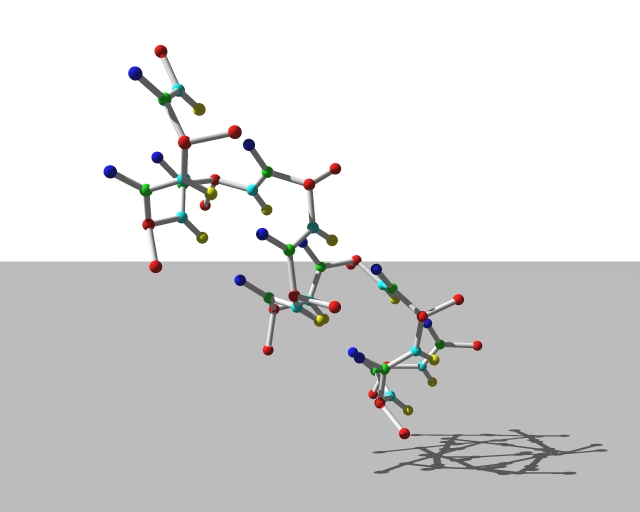
\includegraphics[width=12cm]{alanin_66.jpg}}
    \caption{Picture of alanin, generated by the BOOGA application \ttsmall{raytrace}.  \label{fig:alanin}}
\end{figure}


%\begin{figure}
 %  \centering
  % \includegraphics[width=5.5cm]{alanin.ps}
   % \caption{Picture of alanin, generated by the BOOGA application \ttsmall{raytrace}.  \label{fig:alanin}}
%\end{figure}


%%%%%%%%%%%%%%%%%%%%%%%%%%%%%%%%%%%%%%%%%%%%%%%%%%%%%%%%%%%%%%%%%%%%%%%%%
\section{20 \AA{ }diameter water droplet With A Two-Level Integration
  Scheme}

This sample of water is being run using a two-level integration scheme,
starting with an MTS Impulse Integrator with a cycle length of 5
and finishing with an STS PLeapFrog Integrator that has a timestep of
0.5.  The initial temperature is 300 and the first timestep is 0, and
the simulation will be run for 200 steps.  Note the cubic cell manager
and periodic boundary conditions, and that all cell basis vectors have
been provided.  Note also that though the user specified a restart
file prefix and a restart frequency, restart files will never be
written because restartfreq at 1000 is higher than the total number of
steps for the simulation.  Output files, however, will be written,
including a DCD trajectory file and an all energies file, every 10
steps.  The final files written will be both a position and velocity
file in XYZ format, and also a final BSDL file.  Note that all
necessary initial data files have been provided.
\clearpage
\begin{verbatim}        
   temperature 300.0 
   firststep 0
   numsteps 200
   cellsize 6.5
   outputfreq 10
   restartfreq 1000      
   seed 1234
   posfile equil298K_01.pos.pdb
   velfile equil298K_01.vel.pdb
   psffile equil298K_01.psf
   parfile equil298K_01.par
   finXYZPOSFILE         equil298K_01.out.fin.pos.xyz
   finXYZVELFILE         equil298K_01.out.fin.vel.xyz
   DCDFILE               equil298K_01.out.trajectory.pos.dcd
   ALLENERGIESFILE       equil298K_01.out.energies
   BSDLFILE              equil298K_01.out.fin.bsdl
   RESTARTFILE           equil298K_01.out.restart
   doRestartFile no
   usecharmm28parfile no
   cellBasisVector1     28.0 0.0 0.0
   cellBasisVector2     0.0 28.0 0.0
   cellBasisVector3     0.0 0.0 28.0
   cellorigin           0.0 0.0  0.0
   boundaryConditions Periodic
   cellManager Cubic
   Integrator {
       level 1 Impulse {
                 cyclelength 5
          force Coulomb
                   -algorithm NonbondedSimpleFull
                   -switchingFunction ComplementC1
                   -cutoff 6.5
        }
        level 0 PLeapfrog {
                 timestep .5
          force Bond, Angle 
          force Coulomb
                   -algorithm NonbondedCutoff
                   -switchingFunction C1
                   -cutoff 6.5
          force LennardJones
                   -algorithm NonbondedCutoff    
                   -switchingFunction C2
                   -cutoff 6.5
                   -switchon 0.1
       }
   }
\end{verbatim}        
\clearpage
\begin{figure}[htb]
   \centerline{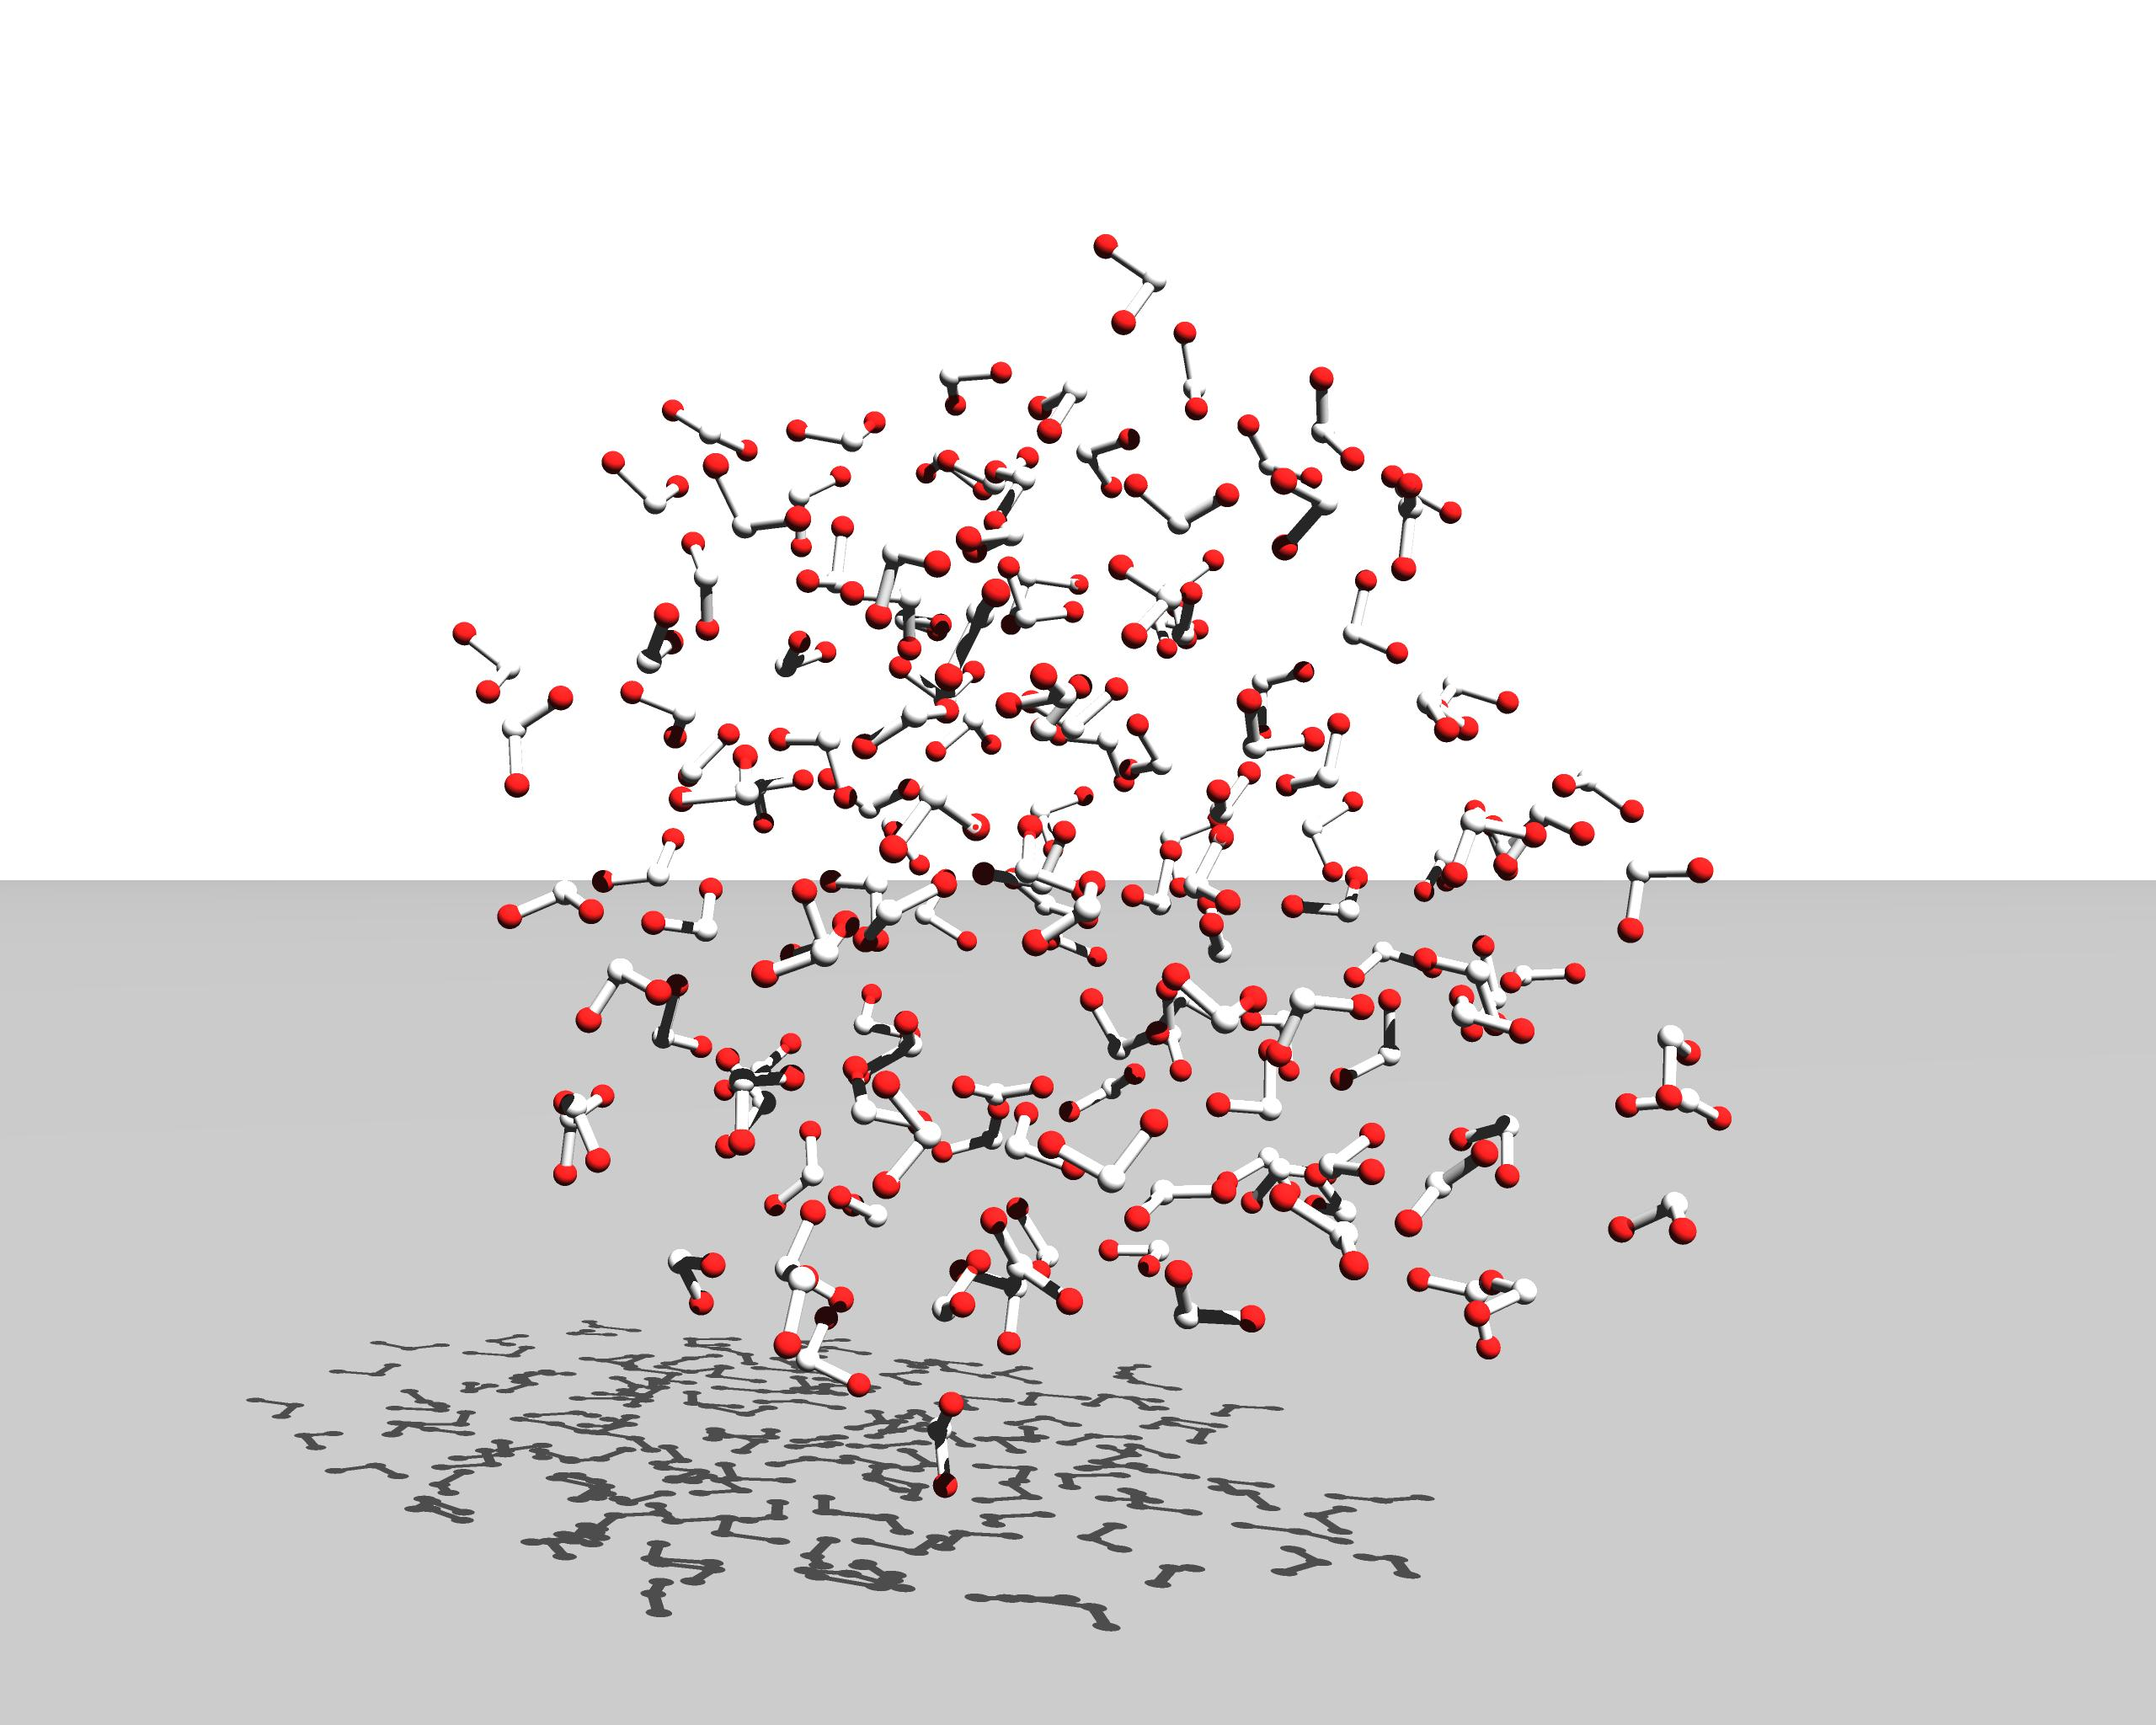
\includegraphics[width=12cm]{water_423.jpg}}
    \caption{Picture of 10 \AA{ }diameter water droplet, generated by the BOOGA application \ttsmall{raytrace}.  \label{fig:water423}}
\end{figure}


%\begin{figure}
 %  \centering
  % \includegraphics[width=5.5cm]{water423.ps}
   % \caption{Picture of 20 \AA{ }diameter water droplet, generated by the BOOGA application \ttsmall{raytrace}.  \label{fig:water423}}
%\end{figure}

%%%%%%%%%%%%%%%%%%%%%%%%%%%%%%%%%%%%%%%%%%%%%%%%%%%%%%%%%%%%%%%%%%%%%%%%%
\section{BPTI with Hybrid Monte Carlo Sampling}

Here is an example of the Hybrid Monte Carlo algorithm used to sample
a BPTI molecule - a 2-level Hybrid Monte Carlo MTS integrator is used.
Once again, the initial timestep is at time 0, but the number of
timesteps to run this time is 100.  1-2 exclusions are desired, and
the cellsize is once again 6.5.  There are now however periodic
boundary conditions, and as a result three cell basis vectors along
with a cell origin are required.  Output files will be written to
every 10 timesteps - this time they include XYZ position and
trajectory files, a DCD trajectory file, an XYZ forces file, and a
split energies file (thus there will be 10 different energy files
generated - one for each type of energy).  The restart files will be
written three times, at 0, 50 and 100 timesteps.  Note that a final
XYZ position file will be written but NOT a final XYZ velocities file
even though the filename was specified; setting dofinxyzvelfile to
``no'' overrides the filename.  Also a final BSDL file -
bpti.out.bsdl3 will be written.  Since commotion is set to ``yes'',
center of mass motion will be removed when calculating velocities.
Once again notice the cubic cell manager, and also notice that the
HMCIntegrator does not have forces.  The integrator will run 5 Hybrid
Monte Carlo cycles, with a cycle length of 10 and 50 warm-up cycles,
at a temperature of 300 K.  Four bonded forces (bond, angle, improper,
dihedral) are present, and one nonbonded (FullEwald, the Coulomb force
solved for using Ewald summation).
\clearpage
\begin{verbatim}        
   firststep 0
   numsteps 100
   exclude 1-2
   cellsize 6.5
   cellbasisvector1  32.0    0    0
   cellbasisvector2     0 32.0    0
   cellbasisvector3     0    0 32.0
   cellorigin           0    0    0
   outputfreq 10
   restartfreq 50
   posfile bpti.pos.pdb
   velfile bpti.vel.xyz
   psffile bpti.psf
   parfile bpti.par
   finxyzposfile bpti.out.pos.xyz
   finxyzvelfile bpti.out.vel.xyz
   dofinxyzvelfile no
   xyzposfile bpti.out.trajectory.pos.xyz
   xyzvelfile bpti.out.trajectory.vel.xyz
   dcdfile bpti.out.dcd
   xyzforcesfile bpti.out.forces.xyz
   doallenergiesfile no
   splitenergiesfile bpti.out.energy
   bsdlfile bpti.out
   restartfile bpti.out
   boundaryConditions Periodic
   commotion yes
   cellManager Cubic
   Integrator {
         level 1 HybridMC {
                 cyclelength 10
                 warmupcycles 50
                 temperature 300.0
      }
         level 0 PLeapFrog {
                 timestep 1
         force Bond, Angle, Dihedral, Improper
         force Coulomb 
            -algorithm FullEwald 
            -real 
            -reciprocal 
            -correction
      }
   }
\end{verbatim}        

%%%%%%%%%%%%%%%%%%%%%%%%%%%%%%%%%%%%%%%%%%%%%%%%%%%%%%%%%%%%%%%%%%%%%%%%%

\chapter{Parallelization}

Parallel communication for \ProtoMol is based on {\it Message Passing
  Interface (MPI)}.  What \ProtoMol uses is an
incremental parallelization scheme for clusters with a moderate number
of nodes, e.g. up to 64 CPUs.  The design is based on a force
decomposition with a master-slave paradigm. \\

The appropriate steps for running \ProtoMol on parallel machines
depends greatly on the machine being used.  On SGI you need to add 
``\ttsmall{mpirun -np <number of nodes>}'' at the beginning
of the command line, and on the IBM Regatta you start \ProtoMol\ by
``\ttsmall{poe ./protomol <protomol arugements> -procs <number of nodes>}''. Otherwise, the
appropriate flags may be set in the compilation of \ProtoMol to
generate an MPI compilation. \\

On some machines a queuing system like LSF or PBS may be necessary.
For more information on this ask your system administrator.

%\begin{figure}[htb]
 %       \begin{minipage}[htb]{8cm} 
  %      \centerline{\includegraphics[width=7.2cm]{transfer.pdf}}
   %     \end{minipage} 
    %    \hfill
     %   \begin{minipage}[htb]{8cm}
      %  \centerline{\includegraphics[width=7.2cm]{memory.pdf}}
      %  \end{minipage}
      %  \caption{(a) The master-slave paradigm\label{fig:transfer}, 
       %          (b) The data (memory) exchange between the master and the slaves.\label{fig:memory}}
%\end{figure}


%%%%%%%%%%%%%%%%%%%%%%%%%%%%%%%%%%%%%%%%%%%%%%%%%%%%%%%%%%%%%%%%%%%%%%%%%

\chapter{Interaction of \ProtoMol with VMD}

You may start VMD normally before you begin running the desired
simulation to be viewed in \ProtoMol.  Select the ``molecule'' option
from the main window, and in the resulting molecule window select
``Load From Files''.  Then in the files window that opens, under the
menu ``Molecule File Types'' select psf and pdb, then write the full
pathnames of the PSF and PDB files used in the simulation that will be
run in the provided spaces.  Now VMD has the initial state of the
molecule to be simulated. \\

Next, in the configuration file that will be used, make sure there is
a Haptic force in the integrator.  Check to see that a positive
nonzero value is supplied for the ``-wait'' value under the haptic
force.  This will force \ProtoMol to wait some time for an IMD
connection, 100 would be a decent value so that you have time to set
VMD to simulate.  Also note the port number, which will be used
later.\\

Now run \ProtoMol.  It should display ``Waiting for IMD
connection.....'' after a short time.  At this point, go to the VMD
console window and type ``\ttsmall{imd connect <hostname> <port
number>}'', where \ttsmall{<hostname>} is the name of the
machine that \ProtoMol is running on and \ttsmall{<port number>}
is the port number value specified in the configuration file that is
being used.\\

At this point, VMD will view the molecule throughout the simulation as
\ProtoMol runs.  Also from the VMD window IMD commands can be run that
will send messages to \ProtoMol.  For example, typing\\ ``\ttsmall{imd
trate <integer value>}'' will change the transmission rate for
information from \ProtoMol to VMD.\\

As an example, let us return to the integrator section of the alanin configuration file from section \ref{sec:alanin}:\\

\begin{verbatim}        
Integrator {
       level 0 Leapfrog {
                timestep 1
         force Improper 
         force Dihedral
         force Bond
         force Angle 
         force LennardJones
                  -algorithm NonbondedCutoff
                  -switchingFunction C2
           -switchon 0.1
                  -cutoff 12
         force Coulomb
                  -algorithm NonbondedCutoff
                  -switchingFunction C1
                  -cutoff 12
         force Haptic
           -port 2001
           -trate 1
           -timeout 1000
           -step_inc 100
           -wait 100
       }
   }
\end{verbatim}        

The only area that counts as far as the VMD simulation is concerned is
the ``\ttsmall{force Haptic}'' section at the end.  Notice first that
a \ttsmall{-wait} value is given that is greater than zero, thus
\ProtoMol will wait for an IMD connection, which is what we want.  The
port ID is 2001.  The other three values are IMD variables. \\ 

In this case as soon as \ProtoMol begins waiting for the IMD
connection, a user would type\\ ``\ttsmall{imd connect <name of the
    machine on which \ProtoMol is running> 2001}'' and the visual
simulation will begin.  Now the user can run IMD commands in the IMD
window while the simulation is running.
\begin{figure}[htb]
   \centerline{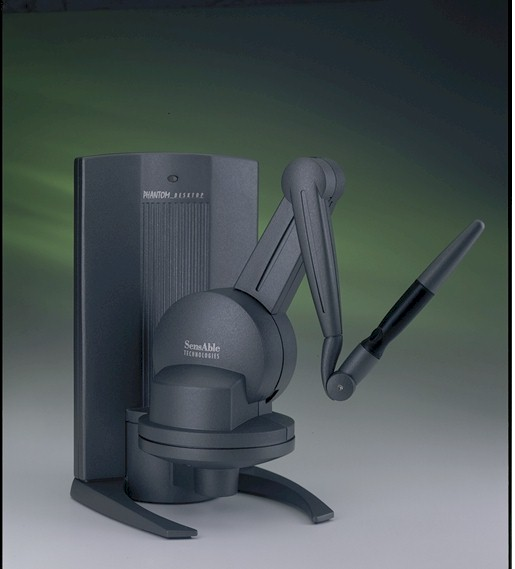
\includegraphics[width=8cm]{hapticdevice.jpg}}
    \caption{ PHANTOM Desktop$^{TM}$ Haptic Device.  \label{fig:hapticdevice}}
\end{figure}


%%%%%%%%%%%%%%%%%%%%%%%%%%%%%%%%%%%%%%%%%%%%%%%%%%%%%%%%%%%%%%%%%%%%%%%%%
\chapter{Availability and Installation of \ProtoMol}

%%%%%%%%%%%%%%%%%%%%%%%%%%%%%%%%%%%%%%%%%%%%%%%%%%%%%%%%%%%%%%%%%%%%%%%%%
\section{How to Download \ProtoMol}

The download site for \ProtoMol is a link from the page for the
Laboratory for Computational Life Sciences at the University of Notre
Dame: \texttt{http://protomol.sourceforge.net/}.
Executable code is available online, and source code will be available
upon request.  An agreement to a Non-Exclusive, Non-Commercial Use
License is required (this exact license can be found in the appendix
of this user guide, appendix B) for download.

%%%%%%%%%%%%%%%%%%%%%%%%%%%%%%%%%%%%%%%%%%%%%%%%%%%%%%%%%%%%%%%%%%%%%%%%%
\section{Platforms that \ProtoMol is Able to Run On}

\ProtoMol executables are available for the following three platforms:

\begin{enumerate}
\item Sun OS 5.8
\item Linux 2.4 
\item IRIX 6.5 (optional with MPI)
\item AIX 5.1 (optional with MPI)
\item HP-UX (optional with MPI)
\item Windows
\end{enumerate}

%%%%%%%%%%%%%%%%%%%%%%%%%%%%%%%%%%%%%%%%%%%%%%%%%%%%%%%%%%%%%%%%%%%%%%%%%
\section{Compiling \ProtoMol}

Because executables are available online, compiling \ProtoMol should
not be necessary unless the user would like to change features.   Here
are the steps for generating the appropriate makefiles on different
platforms:


\begin{enumerate}

\item Change to the main {\bf protomol} directory.

\item View the \ttsmall{README} file for specific directions on how to
compile \ProtoMol correctly on the apporpriate platform.

\end{enumerate}


Once the makefiles have been generated, the user types
``\ttsmall{make}'' from the protomol directory.  A ``\ttsmall{make
clean}'' will clear all object files and executables recursively
throughout the directory tree, if necessary.\\


After everything has compiled successfully, the user may run \ProtoMol
from the\newline \ttsmall{protomol/applications/protomol-app} directory
as described in Chapter 2.

%%%%%%%%%%%%%%%%%%%%%%%%%%%%%%%%%%%%%%%%%%%%%%%%%%%%%%%%%%%%%%%%%%%%%%%%%
\section{Documentation}
Available documentation for \ProtoMol can be downloaded from:\\
\\
\ttsmall{http://protomol.sourceforge.net/}

%%%%%%%%%%%%%%%%%%%%%%%%%%%%%%%%%%%%%%%%%%%%%%%%%%%%%%%%%%%%%%%%%%%%%%%%%
\chapter{The Future of \ProtoMol}

Work is already under way to further exapand \ProtoMol.  In the next
few years, various new algorithms will be placed in the back end,
including new MOLLY integrators and semi-implicit integrators using iterative solvers and sparse matrices, rigid body dynamics, and table lookups.  The goal is to acheive larger
time steps and thus decrease the amount of time necessary to run a
simulation. \\


The \ProtoMol design team is also looking into automated
empirical optimization of the software (AEOS) for optimal parameters and
algorithm selection.  With this implementation, the software could
automatically generate an extremely efficient simulation, enhancing both
usability and speed. \\

Additionally, the next release of \ProtoMol will hopefully
include a graphical interface, again increasing ease of use.  The
program is currently being ported to Windows and will be released in the
near future.


%%%%%%%%%%%%%%%%%%%%%%%%%%%%%%%%%%%%%%%%%%%%%%%%%%%%%%%%%%%%%%%%%%%%%%%%%
\begin{appendix}

%%%%%%%%%%%%%%%%%%%%%%%%%%%%%%%%%%%%%%%%%%%%%%%%%%%%%%%%%%%%%%%%%%%%%%%%%
\chapter{Background}

%%%%%%%%%%%%%%%%%%%%%%%%%%%%%%%%%%%%%%%%%%%%%%%%%%%%%%%%%%%%%%%%%%%%%%%%%
\section{Integrators}

MD describes a molecular system as a function of time based on the
integration of Newton's equations of motion and interacting forces.  The
integrators are the part of the program that that solve the differential
equations that describe the system.  Specifically, the integrators provide a set of
forces, velocities, positions, etcetera, that describe the system at each
time step.  Thus, it is easy to see that the central part of the entire
system is the integrators:  the front end reads in data and passes it to
the integrators, then the integrators call the back end's high performance
functions to do the massive computations.  The way those computations are
assembled into useful data describes the integrator. \\ \\ \\

%%%%%%%%%%%%%%%%%%%%%%%%%%%%%%%%%%%%%%%%%%%%%%%%%%%%%%%%%%%%%%%%%%%%%%%%%
\subsection{Standard integrators in \ProtoMol}
\label{sec:standardintegrator}

For \ProtoMol, a standard integrator is one that updates the velocities by half a step, updates the positions, calculates forces, and finally updates the velocities by another half a step.  This method is noted in \ProtoMol as:
\begin{itemize}
\item \textit{ halfkick();}
\item \textit{ doDriftOrNextIntegrator();}
\item \textit{ calculateForces();}
\item \textit{ halfkick();}
\end{itemize}

%%%%%%%%%%%%%%%%%%%%%%%%%%%%%%%%%%%%%%%%%%%%%%%%%%%%%%%%%%%%%%%%%%%%%%%%%
\subsection{Distinction between multiple-time-stepping (MTS) and single-time-stepping (STS) integrators}

Because of the massive amounts of computation for very large systems
(as are found in MD), it is essential to have more sophisticated ways
of integration than to just use a single time unit per step.  With an
STS integrator, one typically takes timesteps of one femtosecond.
This small of a timestep would however not be feasable for long
simulations with many atoms since useful simulations are typically run
for somewhere in the range of one microsecond to one second.  This can
mean literally months of computations on the computer.  Thus, MTS
integrators are desired since they are capable of taking longer
timesteps. \\


When running \ProtoMol, the integrator at level 0 (or terminating
integrator) must be STS.  Looking at the sequence of standard
integrator operations in section \ref{sec:standardintegrator}, when an MTS integrator calls
{\it doDriftOrNextIntegrator()}, it looks for an MTS or STS integrator
that is next in the chain to run.  But when an STS integrator calls
this function, it actually updates the positions, calculates the
forces, updates the velocities and returns.  Therefore because an STS
integrator does not look for a following integrator, it must not have
one.  Thus an STS integrator in \ProtoMol must be at level 0, while an
MTS integrator can never be at that level. \\


%%%%%%%%%%%%%%%%%%%%%%%%%%%%%%%%%%%%%%%%%%%%%%%%%%%%%%%%%%%%%%%%%%%%%%%%%
\subsection{The Verlet-I/r-RESPA Impulse Method ~\cite{Izag99}} 

The {\it Impulse} method is a MTS method for solving Newton's
equations of motion and is supported by \ProtoMol.  The first step is
to separate the system force into a fast and slow part, each with
their own distinct timesteps.  Bonded terms have the fastest normal
modes in the system and are thus classified as fast.  Nonbonded terms,
both Lennard Jones and electrostatic, are split into fast and slow
depending on range (short-range is fast, long-range is slow).  With
appropriate bonded conditions, the fast part becomes cheap to
integrate compared to the cost of integrating the full system, since
only short-range forces are considered.  Long-range forces
(electrostatic forces beyond 8 \AA{ }) need to be evaulated sparingly
for efficiency purposes.  The impulse method ``approximates the slow
force by a sequence of impulses with weights {\begin{math} \Delta
\end{math}}t dictated by consistency.''   Analytical evaluation of the
fast forces can be avoided using a similar method - a sequence of
suitably weighted impulses that are more closely spaced in time than
the slow force impulses.  The method as a whole can be described by
the following equation: \\

\begin{equation}
M \frac{{\mathrm{d}}^2} {\mathrm{d} t^2} X = \sum_{n'=-\infty}^{\infty} \delta t {\bf \delta} (t - n'\Delta t) {F}^{fast} (X) + \sum_{n=-\infty}^{\infty} \Delta t {\bf \delta}(t - n\Delta t) {F}^{slow} (X)
\end{equation}


%%%%%%%%%%%%%%%%%%%%%%%%%%%%%%%%%%%%%%%%%%%%%%%%%%%%%%%%%%%%%%%%%%%%%%%%%
\subsection{Mollified Impulse Methods (\MOLLY) ~\cite{Izag99}}

\MOLLY is a family of integrators~\cite{GaSS98b} that counteracts the
instabilities and accuracy reduction present in the multiple time
stepping Verlet-I/r-RESPA 
integrator. This is accomplished by perturbing the potential using
time averaged positions
\begin{equation}
U^{{\rm slow}}(X)\rightarrow U^{{\rm slow}}({\mathcal{A}}(X)),
\end{equation}
with the force defined as a gradient of this averaged potential, 
\begin{equation}
-\nabla U^{{\rm slow}}(X)\rightarrow -{\mathcal A}_{X}(X)^{{\rm T}}\nabla U^{
{\rm slow}}({\mathcal A}(X)).
\end{equation}

This perturbation is supposed to compensate for finite $\Delta t$
artifacts.  Perturbing the potential rather than the force ensures
that the numerical integrator remains symplectic \cite{SaCa94}. The
force used by \MOLLY is the gradient of the perturbed potential
\cite{IzRS99}. \MOLLY can be seen as a filter that eliminates
components of the slow force impulse in the directions of the fast
forces, and thus improves the stability of Verlet-I/r-RESPA. Different
averaging functions give rise to MOLLY integrators with different
stability and accuracy properties. 

\begin{itemize}

\item {\bf Equilibrium MOLLY - ~\cite{IZAG98}}
 Here we present a time averaging
completely eliminate the components of $-U_{x}^{ {\rm slow}}$ in the
directions of the fast forces. Our starting point is the backward
Euler averaging:
\begin{equation}
{\mathcal A}(x)=x-\Delta t^{2}M^{-1}U_{x}^{\rm fastest}({\mathcal A}(x)),
\end{equation}
which is obtained with one step of backward Euler starting
with zero velocities. 

Assume that $U^{\rm fastest}$ can be written as 
$U^{\rm fastest}=\chi (g(x)),$ 
where $g(x)$ is a vector of independent length constraint functions. 
The elements of $g(x)$ are of the form
\begin{equation}
g^{k}(x)=x^{\mathrm{T}}G_{k}x-l_{k}^{2},
\end{equation}
where the $G_{k}$ are symmetric matrices and $l_k$ are rest lengths. 
Both $U^\mathrm{bond}$ and $U^\mathrm{angle}$ can be expressed in the
form $\chi(g(x))$. Allowing $\Delta t\rightarrow \infty $ gives the
equations for 
${\mathcal A}(x)$ and $\mu$ 
\begin{equation}
\left\{ 
\begin{array}{c}
M({\mathcal A}(x)-x)+g_{x}^{{\rm T}}({\mathcal A}(x))\mu =0, \\ 
g({\mathcal A}(x))=0,
\end{array}
\right\}.  
\label{eq:ultrazero}
\end{equation}
which are termed {\em Equilibrium*}; this method completely eliminates
components of $-\nabla U^{{\rm slow}}$ in the directions of the
constraints $ g_{x}^{{\rm T}}.$ A proof of the stability of {\em
Equilibrium*} for a general linear model problem under the assumption
that all the fast forces are included in the mollification ($U^{ {\rm
fastest}}=U^{{\rm fast}}$) is given in Ref.~\cite{Izag99b}. An
earlier version is in Ref.~\cite{Reic98}. 

The stability condition for {\em
Equilibrium*} MOLLY on the longest time step 
\begin{equation}
\Delta t\rho(M^{-1/2}U_{xx}^{{\rm slow}}M^{-1/2})^{1/2}<2,
\end{equation}
where $\rho$ is the spectral radius of the mass weighted Hessian
matrix $M^{-1/2}U_{xx}^{{\rm slow}}M^{-1/2}$, is less restrictive than
that of the popular leapfrog integrator:
\begin{equation}
\Delta t\rho(M^{-1/2}U_{xx}M^{-1/2})^{1/2}<2,
\end{equation}
because it is limited by the
fastest frequencies in the slow forces ($-\nabla U^{{\rm slow}}$)
rather than by the overall fastest frequencies (in $-\nabla U^{{\rm
fast}}$).
\\ \\

\item {\bf BSpline MOLLY - ~\cite{IZAG98}} 
It is possible to use time averagings that consist of numerically integrating
an auxiliary, reduced problem:
\begin{equation}
\mathcal{A}(x)=\frac{1}{\Delta t}\int_{0}^{\infty}\phi\left(  \frac{t}{\Delta
t}\right)  \tilde{X}(t)dt \label{eq:weightave}
\end{equation}
where $\phi\left(  \frac{t}{\Delta t}\right)  $
\index{01w0phifun@$\phi(s)\mathcal{\qquad}$\ Weight function of compact
support} is a weight function, and $\tilde{X}(t)$
\index{02X2XTILDE@$\tilde{X}\mathcal{\qquad}$\ Positions for auxiliary
problem} solves an \emph{auxiliary} problem
        \begin{equation}
M\frac{\mathrm{d}^{2}}{\mathrm{d}t^{2}}\tilde{X}=F^{\mathrm{reduced}}
(\tilde{X}),\quad\tilde{X}(0)=x,\quad\frac{\mathrm{d}}{\mathrm{d}t}\tilde
{X}(0)=0. \label{eq:reducedflow}
\end{equation}

This approach is computationally feasible if the weight functions
$\phi$ have compact support in time. The paper~\cite{GaSS98b} suggests
using B-spline weight functions, which are non-zero over a short
interval. The effectiveness of the averagings induced by these weight
functions is directly related to the extensiveness of the time
averaging. One such B-spline weight function that has been tested is
called LongAverage:

\begin{equation}
\phi(s) = \begin{cases}
        0, & \quad s < 0,       \\
        1, & \quad 0 \leq s < 1,\\
        \frac{1}{2}, & \quad s = 1 \\
        0, & \quad s > 1.
        \end{cases}
\label{eq:bspline00}
\end{equation}

The coding of $\mathcal{A} (x)$ and
$\mathcal{A}_{x}(x)$ can be done by hand in a systematic
manner. First the calculation of $\mathcal{A}(x)$ is coded, and then
the differentiation, applying the chain rule with respect to each of
the components of $x$ to yield code for $\mathcal{A}_{x}(x)$. As an
example suppose that the leapfrog method with time step $\delta t$ is
coded for the calculation of $\mathcal{A}(x)$. This is then
differentiated to obtain $\mathcal{A}_{x}(x)$.  The result is the
following code for calculating $\mathcal{A}(x)$ and
$\mathcal{A}_{x}(x)$:

Initialization is given by
\begin{equation}
\begin{array}[c]{cc}
X:=x, & X_{x}:=I,\\
P:=0, & P_{x}:=0,\\
B:=0, & B_{x}:=0, \\
t:=0, & 
\end{array}
\end{equation}
and step by step integration by
\begin{equation}
\begin{array}[c]{ll}
P:=P+\frac{1}{2}\delta tF^{\mathrm{reduced}}(X), & P_{x}:=P_{x}+\frac{1}
{2}\delta tF_{x}^{\mathrm{reduced}}(X)X_{x},\\
B:=B+\frac{1}{2}\delta tX\phi(t/\Delta t), 
& B_{x}:=B_{x}+\frac{1}{2}\delta tX_{x} \phi(t/\Delta t),\\
X:=X+\delta tM^{-1}P, & X_{x}:=X_{x}+\delta tM^{-1}P_{x},\\
t:= t+\delta t, & \\
B:=B+\frac{1}{2}\delta tX\phi(t/\Delta t), 
& B_{x}:=B_{x}+\frac{1}{2}\delta tX_{x}\phi(t/\Delta t),\\
P:=P+\frac{1}{2}\delta tF^{\mathrm{reduced}}(X), & P_{x}:=P_{x}+\frac{1}
{2}\delta tF_{x}^{\mathrm{reduced}}(X)X_{x}.
\end{array}
\end{equation}
The value $(1/\Delta t)B$ is used for $\mathcal{A}(x)$ and $(1/\Delta
t)B_{x}$ for $\mathcal{A}_{x}(x)$. We continue the above integration
until we reach a value of $t$ such that $\phi(t/\Delta t)$ is zero at
this value and remains zero for larger values of $t.$ In practice, one
can choose $\delta t$ equal to the stepsize of the lowest
level integrator. 
In the above loop, $F_x = - U^\mathrm{reduced}_{xx}(x)$ must be
computed efficiently. We have derived the
analytical form of the Hessian matrices, $U^\mathrm{reduced}_{xx}(x)$ \cite{IzMa01}.


\item {\bf H-Bond MOLLY - ~\cite{IzagCar00}} A large part of using
\MOLLY is to determine which forces need to be included in the time
averaging.  Systems that are particularly sensitive to instability are
those dissolved in water.  Water is a hydrogen bonded system, and the
presence of hydrogen bonds accounts for many important properties of
liquid water, proteins, and their interactions.  It has been found
that hydrogen bond interactions are very important terms to
include in the time averaging.  H-Bond \MOLLY uses not only the bonds
and angles in the averaging, but also the H-Bonds which are modeled by 
the nonbonded short range Coulomb and LennardJones forces, and thus
presents itself as a superior integrator, even to Equilibrium.

A straightforward implementation of B-spline \MOLLY and H-Bond
\MOLLY would compute the filter matrix,
$\mathcal{A}(x)$ directly, which involves sparse matrices and
multiplies of those sparse matrices. Another way to implement these
two methods is to construct the filter matrix implicitly and
completely get rid of sparse matrix multiplies using a linear
approximation of $\mathcal{A}(x)$. A more detailed description of the
efficient implementation of H-Bond \MOLLY is available on line\\
(\ttsmall{http://www.cse.nd.edu/\~{ }lcls/docs/fastHbond/}).

\end{itemize}

%%%%%%%%%%%%%%%%%%%%%%%%%%%%%%%%%%%%%%%%%%%%%%%%%%%%%%%%%%%%%%%%%%%%%%%%%
\section{Forces}

Forces define the interaction between the atoms. Newton's equations of
motion, which are solved by the integrators for the interacting atoms, evaluate
these forces to calculate new positions and velocities. On
a given atom at
position $\vec{r_{i}}$,
\begin{equation}
 m_{i} \vec{\ddot{r_{i}}} =  \vec{F_{i}} = \sum_{j=1,j \neq i}^{N} -\nabla
 U(\vec{r}_{ij}).
\end{equation}
   Here $m_{i}$ is the mass of particle $i$ and $r_{ij}$ is the distance
between particle $i$ and $j$. The complexity of the force calculation
is governed by the potential function $U(\vec{r}_{ij})$.
\\

In \ProtoMol, forces are held by the integrators and can be removed or added dynamically.  \ProtoMol makes distinctions between system forces and extended forces, as well as non-bonded and bonded forces.



%%%%%%%%%%%%%%%%%%%%%%%%%%%%%%%%%%%%%%%%%%%%%%%%%%%%%%%%%%%%%%%%%%%%%%%%%
\subsection{Bond force}

Bonds~\cite{NELS96} describe a linear bond between two atoms. These bonds are
described by a simple harmonic spring. The energy of a bond between
atoms $i$ and $j$ is given by:

\begin{equation}
E_{bond} = k \left( \left| \vec{r}_{ij} \right| - r_0 \right)^2   \label{eq:BondEnergy}
\end{equation}

\noindent
where\\

\begin{tabular}{lcl}
 $ k $      & = & Spring constant specified in the parameter file for this bond type.\\
 \Vr{ij}    & = & \Vr{j} - \Vr{i} \\
 \AbsVr{ij} & = &  $ \sqrt{(x_j - x_i)^2 + (y_j - y_i)^2 + (z_j - z_i)^2} $ \\
            & = & calculated distance between atoms $i$ and $j$.\\
 $ r_0 $    & = & Rest distance of the bond specified in the parameter file for this bond type.
\end{tabular}
\\

By differentiating this formula, the force for this bond can be found to be:
\begin{equation}
\vec{F}_{bond} = - \frac{\mathrm{d} E_{bond}}{\mathrm{d}\vec{r}} 
               = 2 k ( \AbsVr{ij} - r_0 ) \hatr{ij}
\label{eq:BondForce}
\end{equation}


%%%%%%%%%%%%%%%%%%%%%%%%%%%%%%%%%%%%%%%%%%%%%%%%%%%%%%%%%%%%%%%%%%%%%%%%%

\subsection{Angle force}

Angles~\cite{NELS96} describe angular bonds between three atoms.
These bonds are modeled as harmonic angular springs. 
The energy of such a bond between atoms $i$, $j$,  and $k$ is given by:
\begin{eqnarray}
  E_{angle}  & = & E_{\theta} + E_{\mathrm{ub}} \label{eq:AngleEnergy} \\
  E_{\theta} & = & k_{\theta} \left( \theta - \theta_0 \right)^2   \\
\label{eq:Eub}
  E_{\mathrm{ub}}     & = & k_{\mathrm{ub}} \left( \AbsVr{ik} - r_{\mathrm{ub}} \right)^2
\end{eqnarray}
\noindent
\\
where\\

\begin{tabular}{lcl}
 $ k_{\theta} $ & =  & Force constant specified in the parameter file for this bond type.\\
 $\theta $ & = &  $\cos^{-1} \left( \frac{ \Vr{ij}\, \cdot \,\Vr{kj}
}{ \AbsVr{ij} \AbsVr{kj} } \right),$ which is equivalent to
$\tan^{-1}(\mbox{$\left| {\Vr{ij} \times \Vr{kj}} \right|$}, \Vr{ij} \cdot \Vr{kj})$ \\
$ \theta_0 $   & = & Rest angle of this bond specified in the parameter file for this angle type.\\
$k_{\mathrm{ub}}$ &=& Urey-Bradley constant, which defaults to zero \\
  \Vr{ik}       & = & \Vr{k} - \Vr{i} \\
  \AbsVr{ik}    & = &  $ \sqrt{(x_k - x_i)^2 + (y_k - y_i)^2 + (z_k - z_i)^2},$
                calculated distance between atoms $i$ and $k$.\\
  $ r_{\mathrm{ub}} $    & = & Rest distance for the Urey-Bradley term.
\end{tabular}


By differentiating this formula, the force for this bond can be found to be:
\begin{equation}
\vec{F}_{angle} = - \frac{\mathrm{d} E_{\mathrm{angle}}}{\mathrm{d} \vec{r}} \label{eq:angleForce}
                = \vec{F}_{\theta} + \vec{F}_{\mathrm{ub}}
\end{equation}
where
\begin{eqnarray*}
\vec{F}_{\theta} = - \frac{\mathrm{d} E_{\theta}}
        {\mathrm{d} \theta} \,\frac{\mathrm{d} \theta}{\mathrm{d} \vec{r} }
                = - 2k_{\theta}(\theta - \theta_0) \,\frac{\mathrm{d}
         \theta}{\mathrm{d} \vec{r} }\\
\vec{F}_{\mathrm{ub}} = - \frac{\mathrm{d} E_{\mathrm{ub}}}
        {\mathrm{d} \vec{r}} = 2 k_{\mathrm{ub}} 
(\AbsVr{ik} - r_{\mathrm{ub}}) \hatr{ik}
\end{eqnarray*}
where $\hatr{ik}$ is the unit vector in the direction of $\vec{r_{ik}}.$


%%%%%%%%%%%%%%%%%%%%%%%%%%%%%%%%%%%%%%%%%%%%%%%%%%%%%%%%%%%%%%%%%%%%%%%%%

\subsection{Dihedral and improper forces}

Dihedral and improper bonds~\cite{NELS96} model the interaction between 4 bonded atoms.  
They are modeled by an angular spring between planes formed by the first
three atoms and the second 3 atoms.  The energy for a dihedral or improper
between atoms $i$, $j$, $k$, and $l$ is given by:

\begin{equation}
  E_{d/i} = \left\{ \begin{array}{ll}
         k \left( 1 + \cos(n \phi + \delta) \right) & \mbox{if $n > 0$} \\
         k \left( \phi - \delta \right)^2          & \mbox{if $n = 0$} 
                    \end{array}
            \right.
\end{equation}

\noindent
Where\\
\begin{tabular}{lcl}
 $k$ & = & Force constant specified in the parameter file for this bond type.\\
 $\phi$ & = &  Calculated angle between the plane formed by atoms $i$, $j$, and $k$ \\
        &   &  and the plane formed by atoms $j$, $k$, and $l$.\\
$n$ & = & Periodicity of the bond specified in the parameter file for this bond type.\\
  $\delta$ & = & Phase shift specified in the parameter file for this bond type.\\
\end{tabular}

\noindent
The angle $\phi$ is calculated by first determining the vectors $\vec{A}$ and $\vec{B}$ where:
\begin{eqnarray*}
  \vec{A} = \Vr{ij} \times \Vr{jk}   \\
  \vec{B} = \Vr{jk} \times \Vr{kl}
\end{eqnarray*}

\noindent
These two vectors can then be used to calculate $\phi$ using the formula,\\

\begin{equation}
  \phi =  \cos^{-1} \left( \frac{ \vec{A} \cdot \vec{B} }{ |\vec{A}| |\vec{B}| } \right)
\end{equation}

\noindent
To determine the force, the negative gradient of the energy must be
found.  It can  be shown that if n$=$0 then the force is given by,
\begin{equation}
  \vec{F} = - 2k \left( \phi - \delta \right) \left( \nabla \phi \right)
\end{equation}

\noindent
and if $n>0$ then the force is given by,\\

\begin{equation}
  \vec{F} = n\,k \sin(n \phi + \delta) \left( \nabla \phi \right)
\end{equation}

\noindent
Using the formula for $\phi$ given, it can be shown that:\\

\begin{equation}
  \nabla \phi =  \frac{ 1 }{ \sin(\phi) } \nabla \left( \frac{ \vec{A}
\cdot \vec{B} }{ |\vec{A}| |\vec{B}| } \right) 
\end{equation}

\noindent
But this can lead to a singularity in $sin( \phi )$ goes to 0.  When
 such a situation has the potential to arise, a third vector $\vec{C}$ 
is determined using

\begin{equation}
        \vec{C} = \Vr{jk} \times \vec{A}
\end{equation}

\noindent
If the angle $\psi$ is the angle between $\vec{C}$ and $\vec{B}$ then 
it can be shown that

\begin{equation}
        \cos( \phi ) = sin ( \psi )
\end{equation}

\noindent
and,

\begin{equation}
        \phi =  sin^{-1} \left( \frac{ \vec{C} \cdot \vec{B} }{ |\vec{C}| |\vec{B}| } \right) + \frac{ \pi }{ 2 }
\end{equation}

\noindent
Therefore

\begin{equation}
  \nabla \phi =  \frac{ 1 }{ \cos(\phi) } \nabla \left( \frac{ \vec{C}
\cdot \vec{B} }{ |\vec{C}| |\vec{B}| } \right) 
\end{equation}



%%%%%%%%%%%%%%%%%%%%%%%%%%%%%%%%%%%%%%%%%%%%%%%%%%%%%%%%%%%%%%%%%%%%%%%%%

\subsection{Non-bonded forces}
Bonded forces define the intramolecular interactions, where non-bonded
forces compromise the intermolecular interactions. Non-bonded
interactions also play an important role in the behavior of individual molecules.
The non-bonded interactions do not depend upon a specific molecular
relationship between atoms. They are usually modeled as a function of
some inverse power of the distance. Non-bonded terms are usually
divided in two groups: one compromising electrostatic and the other
van der Waals interactions. \\

\ProtoMol provides a wide range of different non-bonded force
evaluations, which can be combined with an arbitrary boundary
condition, switching function and potential. Decoupling the algorithm
to compute a given force from the boundary condition, switching
function and potential, we achieve flexibility and performance.  We
template the forces for boundary conditions, switching functions and
potentials. \\ \\

\paragraph{van der Waals forces~\cite{EnBr00}}

 van der Waals forces are ``relatively weak electric forces that attract
neutral molecules to one another in gases, in
liquefied and solidified gases, and in almost
all organic liquids and solids. The forces are
named for the Dutch physicist Johannes van der
Waals, who in 1873 first postulated these
intermolecular forces in developing a theory to
account for the properties of real gases. Solids
that are held together by van der Waals forces
characteristically have lower melting points and
are softer than those held together by the
stronger ionic, covalent, and metallic bonds.\\

Van der Waals forces may arise from three sources. First, the
molecules of some materials, although electrically neutral,
may be permanent electric dipoles. Because of fixed
distortion in the distribution of electric charge in the very
structure of some molecules, one side of a molecule is always
somewhat positive and the opposite side somewhat negative.
The tendency of such permanent dipoles to align with each
other results in a net attractive force. Second, the presence
of molecules that are permanent dipoles temporarily distorts
the electron charge in other nearby polar or nonpolar
molecules, thereby inducing further polarization. An additional attractive force results from the
interaction of a permanent dipole with a neighboring induced
dipole. Third, even though no molecules of a material are
permanent dipoles (e.g., in the noble gas argon or the
organic liquid benzene), a force of attraction exists between
the molecules, accounting for condensing to the liquid state
at sufficiently low temperatures.\\

The nature of the attractive force in molecules, which
requires quantum mechanics for its correct description, was
first recognized (1930) by the Polish-born physicist Fritz
London, who traced it to electron motion within molecules.
London pointed out that at any instant the center of negative
charge of the electrons and the center of positive charge of
the atomic nuclei would not be likely to coincide. Thus, the
fluctuation of electrons makes molecules time-varying
dipoles, even though the average of this instantaneous
polarization over a brief time interval may be zero. Such
time-varying dipoles, or instantaneous dipoles, cannot orient
themselves into alignment to account for the actual force of
attraction, but they do induce properly aligned polarization
in adjacent molecules, resulting in attractive forces. These
specific interactions, or forces, arising from electron
fluctuations in molecules (known as London forces, or
dispersion forces) are present even between permanently polar
molecules and produce, generally, the largest of the three
contributions to intermolecular forces.'' \\

A common and well known approximation for the van der Waal forces is the
general Lennard-Jones 6-12 (LJ) potential
\begin{equation}
      u(r_{ij}) =
          4\epsilon\left[\left(\frac{\alpha}{r_{ij}}\right)^{12} -
            \left(\frac{\beta}{r_{ij}}\right)^{6}\right]
    \label{eq:lennardjones}.
\end{equation}
where $\epsilon$, $\alpha$ and $\beta$ are LJ parameters with $\alpha
\approx \beta$, often is $\alpha = \beta$, it is called $\sigma$. The
potential $u(r_{ij})$ is mostly cutoff at $r_{\mbox{\tiny cutoff}}$
without major loss of accuracy, i.e. no
interactions are evaluated beyond this distance. Since the cutoff
violates assumptions for a simplectic integrator, switching functions
are introduced to smooth the potential at the cutoff. \\ \\
                                         

\paragraph{Coulomb force~\cite{EnBr00}}

 ``also called coulomb interaction, attraction or repulsion of
 particles or objects because of their electric charge. One of
 the basic physical forces, the electric force is named for a
 French physicist, Charles-Augustin de Coulomb, who in 1785
 published the results of an experimental investigation into
 the correct quantitative description of this force.\\

 Two like electric charges, both positive or both negative,
 repel each other along a straight line between their centers.
 Two unlike charges, one positive, one negative, attract each
 other along a straight line joining their centers. The
 electric force is operative between charges down to distances
 of at least $10^{-16}$ meter, or approximately one-tenth of the
 diameter of atomic nuclei. Because of their positive charge,
 protons within nuclei repel each other, but nuclei hold
 together because of another basic physical force, the strong
 interaction, or nuclear force, which is stronger than the
 electric force. Massive, but electrically neutral,
 astronomical bodies such as planets and stars are bound
 together in solar systems and galaxies by still another basic
 physical force, gravitation, which though much weaker than
 the electric force, is always attractive and is the dominant
 force at great distances. At distances between these
 extremes, including the distances of everyday life, the only
 significant physical force is the electric force in its many
 varieties along with the related magnetic force.\\

 The magnitude of the electric force $F$ is directly
 proportional to the amount of one electric charge, $q_i$,
 multiplied by the other, $q_j$, and inversely proportional to
 the square of the distance r between their centers. Expressed
 in the form of an equation, this relation, called Coulomb's
 law, may be written by including the proportionality factor $k$
 as $F = kq_{i}q_{j}/|r_i - r_j|$. In the centimeter-gram-second system of
 units, the proportionality factor $k$ in a vacuum is set equal
 to 1 and unit electric charge is defined by Coulomb's law.''


%%%%%%%%%%%%%%%%%%%%%%%%%%%%%%%%%%%%%%%%%%%%%%%%%%%%%%%%%%%%%%%%%%%%%%%%%

%\subsection{Ewald summation}

%%%%%%%%%%%%%%%%%%%%%%%%%%%%%%%%%%%%%%%%%%%%%%%%%%%%%%%%%%%%%%%%%%%%%%%%%

% The potential energy function per cubic cell of a system of $N$ particles
%interacting with a potential $\phi (\mathbf{r}_{ij}+L\mathbf{n)}$ under
%periodic boundary conditions is usually expressed as the following sum: 
%\begin{equation}
%U=\frac{1}{2}\sum_{\mathbf{n}}\,^{\prime }\left[
%\sum_{i=1}^{N}\sum_{j=1}^{N}\phi (\mathbf{r}_{ij}+\mathbf{n)}\right] 
%\label{eq:total}
%\end{equation}
%where the sum over $\mathbf{n}$ is the sum over all cubic lattice points of
%length $L\nolinebreak =\nolinebreak 1$with integer coordinates $\mathbf{n=}
% (n_{x},n_{y},n_{z})$, the prime over the sum indicates that if $i=j$ the
%terms with $\mathbf{n=0}$ are omitted; and $\mathbf{r}_{ij}=r_{j}-r_{i}$ is
%the distance between particles $i$ and $j.$ \\


%%%%%%%%%%%%%%%%%%%%%%%%%%%%%%%%%%%%%%%%%%%%%%%%%%%%%%%%%%%%%%%%%%%%%%%%%

\section{Switching Functions}
\ProtoMol allows the cutting off of non-bonded forces (electrostatic or van der
Waals) to be handled in two ways. One way is to simply truncate the forces at
the cutoff value, i.e. no interactions are evaluated beyond this distance.  But
this method leads to a discontinuity in the force field and it will violate
energy conservation for symplectic integrators.  The other way of handling
cutoffs are switching functions. These functions smoothly bring the forces and
energies to 0 at the cutoff distance to avoid any discontinuities in the force
field. \\


%%%%%%%%%%%%%%%%%%%%%%%%%%%%%%%%%%%%%%%%%%%%%%%%%%%%%%%%%%%%%%%%%%%%%%%%%

\section{Boundary Conditions}
Boundary conditions define the size of the simulation area and how
atoms will be treated when reaching or crossing boundaries. The most
common area is a cubic box of a finite region.\\
  
Vacuum boundary conditions have no restrictions on the dimension of the
enclosing lattice.  For some applications, the ions and the molecules/atoms can
move in every dimension freely.  Simulations requiring no periodic boundaries
are best suited to simulation in vacuum, such as the conformational study of an
isolated polymer molecule.  Vacuum boundary conditions are not recommended for
studies in a solvent, since evaporation is likely to be a problem.  Note that
vacuum boundary conditions cannot be used with the Ewald summation method. \\

Periodic boundary conditions (PBC) replicate the simulation box
through space to form an infinite lattice. For some applications, the
PBC may be defined only for some dimensions. PBC use the minimal
image convention, whenever an atom moves out of the minimal image it
moves in on the opposite of the minimal image. PBC in all dimesions can
be used with the Ewald summation method. \\

Spherical boundary conditions (SBC) causes a force that moves atoms
back in to (away from) the center of the sphere depending on the force
constant. It may be desirable, however, to simulate a surface tension
affect, where a small harmonic well around the sphere boundary is
desired. To obtain such an effect, two SBC  can be superimposed.


%%%%%%%%%%%%%%%%%%%%%%%%%%%%%%%%%%%%%%%%%%%%%%%%%%%%%%%%%%%%%%%%%%%%%%%%%

\section{Cell Manager}
The cell manager is implemented to achieve better
performance. They control which atom belongs to which cell and store
spatial information of the atom positions, such that the particle's
neighbors can be quickly located for the force
calculation.  Thus, the number of interactions evaluated is
minimized.\\

The multi-cell algorithm uses cells together with a
cutoff, where the cells are cubic and the dimension of the cells are
equal or more than the cutoff. \\ \\ \\ \\ \\ \\
\begin{figure}[htb]
   \centerline{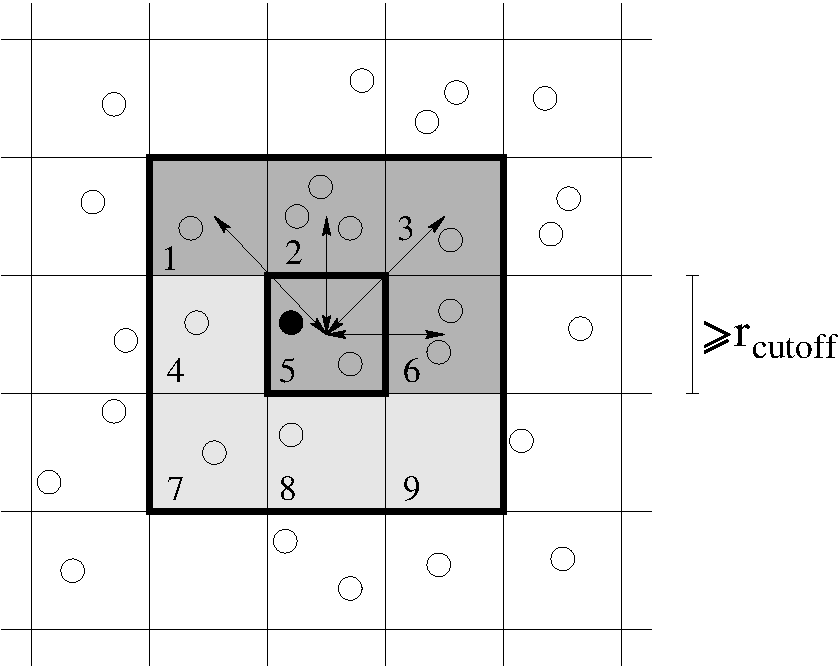
\includegraphics[width=12cm]{cell_algo_cell.pdf}}
    \caption{Partition of cells, where cell no. 5 is the
    origin and 1-4, 6-9 the neighbor cells. Cell no. 6, 3, 2 and 1
    describe the interaction path.\label{fig:cell_algo_cell}}
\end{figure}

%\begin{figure}
 %  \centering
  % 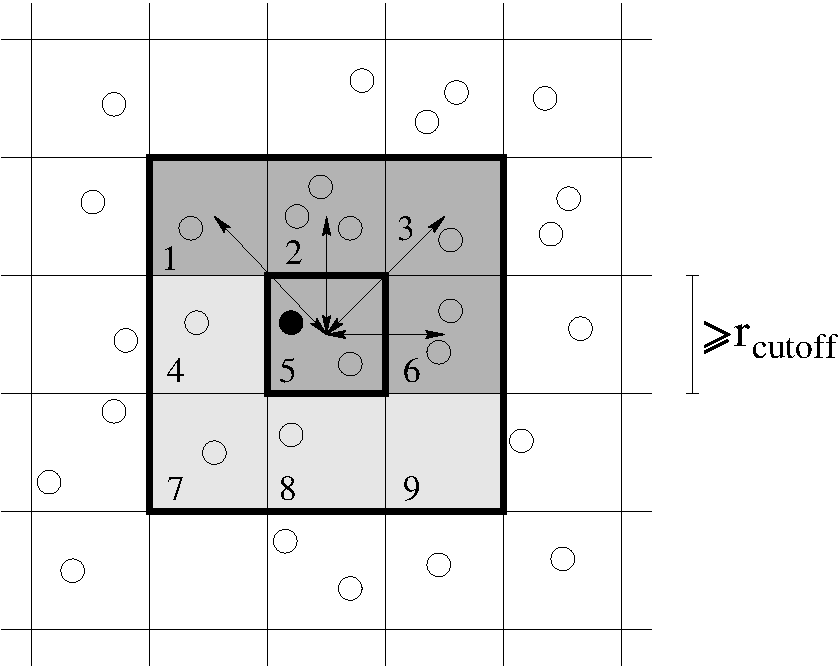
\includegraphics[width=5.5cm]{cell_algo_cell.pdf}
   %\caption{Partition of cells, where cell no. 5 is the
    %origin and 1-4, 6-9 the neighbor cells. Cell no. 6, 3, 2 and 1
    %describe the interaction path.\label{fig:cell_algo_cell}} 
%\end{figure}

\newpage

%%%%%%%%%%%%%%%%%%%%%%%%%%%%%%%%%%%%%%%%%%%%%%%%%%%%%%%%%%%%%%%%%%%%%%%%%

\chapter{\ProtoMol Molecular Dynamcis Software License}

%%%%%%%%%%%%%%%%%%%%%%%%%%%%%%%%%%%%%%%%%%%%%%%%%%%%%%%%%%%%%%%%%%%%%%%%%
\section{Conditions and Regulations}
\footnotesize
\begin{verbatim}
ProtoMol GNU GENERAL PUBLIC LICENSE

This Software is copyrighted by the University of Notre Dame and the University
of Bergen, Norway, whom grant you the right to use this software under
the terms of the GNU General Public License. Although you are under no
obligation, the ProtoMol devlopment team would appreciate the
inclusion of the following citation in all research and development
works which utilize this software:

T. Matthey, T. Cickovski, S. Hampton, A. Ko, Q. Ma, T. Slabach
and J. A. Izaguirre, 'ProtoMol, an Object-Oriented Framework for Prototyping
Novel Algorithms for Molecular Dynamics', ACM Transactions on Mathematical
Software, Vol 30, Num 3, pg 237-265, 2004

               GNU GENERAL PUBLIC LICENSE

   Version 2, June 1991

Copyright c
             1989, 1991 Free Software Foundation, Inc.
59 Temple Place, Suite 330, Boston, MA 02111-1307 USA
Everyone is permitted to copy and distribute verbatim copies of this license
document, but changing it is not allowed.

Preamble
The licenses for most software are designed to take away your freedom to
share and change it. By contrast, the GNU General Public License is in-
tended to guarantee your freedom to share and change free software-to
make sure the software is free for all its users. This General Public Li-
cense applies to most of the Free Software Foundation's software and to any
other program whose authors commit to using it. (Some other Free Software
Foundation software is covered by the GNU Library General Public License
instead.) You can apply it to your programs, too.
   When we speak of free software, we are referring to freedom, not price.
Our General Public Licenses are designed to make sure that you have the
freedom to distribute copies of free software (and charge for this service if
you wish), that you receive source code or can get it if you want it, that you
can change the software or use pieces of it in new free programs; and that
you know you can do these things.
   To protect your rights, we need to make restrictions that forbid anyone to
deny you these rights or to ask you to surrender the rights. These restrictions
translate to certain responsibilities for you if you distribute copies of the
software, or if you modify it.
   For example, if you distribute copies of such a program, whether gratis
or for a fee, you must give the recipients all the rights that you have. You
must make sure that they, too, receive or can get the source code. And you
must show them these terms so they know their rights.
   We protect your rights with two steps: (1) copyright the software, and
(2) offer you this license which gives you legal permission to copy, distribute
and/or modify the software.


   Also, for each author's protection and ours, we want to make certain that
everyone understands that there is no warranty for this free software. If the
software is modified by someone else and passed on, we want its recipients
to know that what they have is not the original, so that any problems
introduced by others will not reflect on the original authors' reputations.
   Finally, any free program is threatened constantly by software patents.
We wish to avoid the danger that redistributors of a free program will in-
dividually obtain patent licenses, in effect making the program proprietary.
To prevent this, we have made it clear that any patent must be licensed for
everyone's free use or not licensed at all.
   The precise terms and conditions for copying, distribution and modifi-
cation follow.

Terms and conditions for copying, distribution and
modification
  0. This License applies to any program or other work which contains a
      notice placed by the copyright holder saying it may be distributed
      under the terms of this General Public License. The "Program", be-
      low, refers to any such program or work, and a "work based on the
      Program" means either the Program or any derivative work under
      copyright law: that is to say, a work containing the Program or a
      portion of it, either verbatim or with modifications and/or translated
      into another language. (Hereinafter, translation is included without
      limitation in the term "modification".) Each licensee is addressed as
      "you".
      Activities other than copying, distribution and modification are not
      covered by this License; they are outside its scope. The act of running
      the Program is not restricted, and the output from the Program is
      covered only if its contents constitute a work based on the Program
      (independent of having been made by running the Program). Whether
      that is true depends on what the Program does.

  1. You may copy and distribute verbatim copies of the Program's source
      code as you receive it, in any medium, provided that you conspicuously
      and appropriately publish on each copy an appropriate copyright no-
      tice and disclaimer of warranty; keep intact all the notices that refer
      to this License and to the absence of any warranty; and give any other



  recipients of the Program a copy of this License along with the Pro-
  gram.
  You may charge a fee for the physical act of transferring a copy, and
  you may at your option offer warranty protection in exchange for a
  fee.

2. You may modify your copy or copies of the Program or any portion
  of it, thus forming a work based on the Program, and copy and dis-
  tribute such modifications or work under the terms of Section 1 above,
  provided that you also meet all of these conditions:

   (a) You must cause the modified files to carry prominent notices stat-
          ing that you changed the files and the date of any change.
   (b) You must cause any work that you distribute or publish, that in
          whole or in part contains or is derived from the Program or any
          part thereof, to be licensed as a whole at no charge to all third
          parties under the terms of this License.
   (c) If the modified program normally reads commands interactively
          when run, you must cause it, when started running for such in-
          teractive use in the most ordinary way, to print or display an
          announcement including an appropriate copyright notice and a
          notice that there is no warranty (or else, saying that you provide
          a warranty) and that users may redistribute the program under
          these conditions, and telling the user how to view a copy of this
          License. (Exception: if the Program itself is interactive but does
          not normally print such an announcement, your work based on
          the Program is not required to print an announcement.)

  These requirements apply to the modified work as a whole. If identifi-
  able sections of that work are not derived from the Program, and can
  be reasonably considered independent and separate works in them-
  selves, then this License, and its terms, do not apply to those sections
  when you distribute them as separate works. But when you distribute
  the same sections as part of a whole which is a work based on the
  Program, the distribution of the whole must be on the terms of this
  License, whose permissions for other licensees extend to the entire
  whole, and thus to each and every part regardless of who wrote it.
  Thus, it is not the intent of this section to claim rights or contest your
  rights to work written entirely by you; rather, the intent is to exercise
  the right to control the distribution of derivative or collective works
  based on the Program.
  In addition, mere aggregation of another work not based on the Pro-
  gram with the Program (or with a work based on the Program) on a
  volume of a storage or distribution medium does not bring the other
  work under the scope of this License.

3. You may copy and distribute the Program (or a work based on it,
  under Section 2) in object code or executable form under the terms of
  Sections 1 and 2 above provided that you also do one of the following:

   (a) Accompany it with the complete corresponding machine-readable
       source code, which must be distributed under the terms of Sec-
       tions 1 and 2 above on a medium customarily used for software
       interchange; or,
   (b) Accompany it with a written offer, valid for at least three years,
       to give any third party, for a charge no more than your cost of
       physically performing source distribution, a complete machine-
       readable copy of the corresponding source code, to be distributed
       under the terms of Sections 1 and 2 above on a medium custom-
       arily used for software interchange; or,
   (c) Accompany it with the information you received as to the offer to
       distribute corresponding source code. (This alternative is allowed
       only for noncommercial distribution and only if you received the
       program in object code or executable form with such an offer, in
       accord with Subsection b above.)

  The source code for a work means the preferred form of the work for
  making modifications to it. For an executable work, complete source
  code means all the source code for all modules it contains, plus any
  associated interface definition files, plus the scripts used to control
  compilation and installation of the executable. However, as a special
  exception, the source code distributed need not include anything that
  is normally distributed (in either source or binary form) with the major
  components (compiler, kernel, and so on) of the operating system on
  which the executable runs, unless that component itself accompanies
  the executable.
  If distribution of executable or object code is made by offering access
  to copy from a designated place, then offering equivalent access to
  copy the source code from the same place counts as distribution of the
  source code, even though third parties are not compelled to copy the
  source along with the object code.

4. You may not copy, modify, sublicense, or distribute the Program ex-
  cept as expressly provided under this License. Any attempt otherwise
  to copy, modify, sublicense or distribute the Program is void, and will
  automatically terminate your rights under this License. However, par-
  ties who have received copies, or rights, from you under this License
  will not have their licenses terminated so long as such parties remain
  in full compliance.

5. You are not required to accept this License, since you have not signed
  it. However, nothing else grants you permission to modify or distribute
  the Program or its derivative works. These actions are prohibited by
  law if you do not accept this License. Therefore, by modifying or
  distributing the Program (or any work based on the Program), you
  indicate your acceptance of this License to do so, and all its terms
  and conditions for copying, distributing or modifying the Program or
  works based on it.

6. Each time you redistribute the Program (or any work based on the
  Program), the recipient automatically receives a license from the orig-
  inal licensor to copy, distribute or modify the Program subject to these
  terms and conditions. You may not impose any further restrictions on
  the recipients' exercise of the rights granted herein. You are not re-
  sponsible for enforcing compliance by third parties to this License.

7. If, as a consequence of a court judgment or allegation of patent in-
  fringement or for any other reason (not limited to patent issues), con-
  ditions are imposed on you (whether by court order, agreement or
  otherwise) that contradict the conditions of this License, they do not
  excuse you from the conditions of this License. If you cannot distribute
  so as to satisfy simultaneously your obligations under this License and
  any other pertinent obligations, then as a consequence you may not
  distribute the Program at all. For example, if a patent license would
  not permit royalty-free redistribution of the Program by all those who
  receive copies directly or indirectly through you, then the only way
  you could satisfy both it and this License would be to refrain entirely
  from distribution of the Program.
  If any portion of this section is held invalid or unenforceable under any
   particular circumstance, the balance of the section is intended to apply
   and the section as a whole is intended to apply in other circumstances.
   It is not the purpose of this section to induce you to infringe any
   patents or other property right claims or to contest validity of any such
   claims; this section has the sole purpose of protecting the integrity of
   the free software distribution system, which is implemented by public
   license practices. Many people have made generous contributions to
   the wide range of software distributed through that system in reliance
   on consistent application of that system; it is up to the author/donor
   to decide if he or she is willing to distribute software through any other
   system and a licensee cannot impose that choice.
   This section is intended to make thoroughly clear what is believed to
   be a consequence of the rest of this License.

 8. If the distribution and/or use of the Program is restricted in certain
   countries either by patents or by copyrighted interfaces, the original
   copyright holder who places the Program under this License may add
   an explicit geographical distribution limitation excluding those coun-
   tries, so that distribution is permitted only in or among countries not
   thus excluded. In such case, this License incorporates the limitation
   as if written in the body of this License.

 9. The Free Software Foundation may publish revised and/or new ver-
   sions of the General Public License from time to time. Such new
   versions will be similar in spirit to the present version, but may differ
   in detail to address new problems or concerns.
   Each version is given a distinguishing version number. If the Program
   specifies a version number of this License which applies to it and "any
   later version", you have the option of following the terms and condi-
   tions either of that version or of any later version published by the
   Free Software Foundation. If the Program does not specify a version
   number of this License, you may choose any version ever published by
   the Free Software Foundation.

10. If you wish to incorporate parts of the Program into other free pro-
   grams whose distribution conditions are different, write to the author
   to ask for permission. For software which is copyrighted by the Free
   Software Foundation, write to the Free Software Foundation; we some-
   times make exceptions for this. Our decision will be guided by the two
   goals of preserving the free status of all derivatives of our free software
   and of promoting the sharing and reuse of software generally.

                                NO WARRANTY

 11. Because the Program is licensed free of charge, there is no
     warranty for the Program, to the extent permitted by ap-
     plicable law. except when otherwise stated in writing the
     copyright holders and/or other parties provide the program
     "as is" without warranty of any kind, either expressed or im-
     plied, including, but not limited to, the implied warranties
     of merchantability and fitness for a particular purpose. The
     entire risk as to the quality and performance of the Program
     is with you. Should the Program prove defective, you assume
     the cost of all necessary servicing, repair or correction.

 12. In no event unless required by applicable law or agreed to
     in writing will any copyright holder, or any other party who
     may modify and/or redistribute the program as permitted
     above, be liable to you for damages, including any general,
     special, incidental or consequential damages arising out of
     the use or inability to use the program (including but not
     limited to loss of data or data being rendered inaccurate or
     losses sustained by you or third parties or a failure of the
     Program to operate with any other programs), even if such
     holder or other party has been advised of the possibility of
     such damages.

               END OF TERMS AND CONDITIONS

\end{verbatim}
\normalsize
%%%%%%%%%%%%%%%%%%%%%%%%%%%%%%%%%%%%%%%%%%%%%%%%%%%%%%%%%%%%%%%%%%%%%%%%%
\section{Contact Information}

The best contact path for licensing issues is by e-mail to  
{\it protomol@cse.nd.edu} or send correspondence to: \\ \\
\ProtoMol Team\\
c/o Prof. Jes\'{u}s A. Izaguirre\\
Laboratory for Computational Life Sciences\\
Department of Computer Science and Engineering\\
University of Notre Dame\\
384 Fitzpatrick Hall of Engineering\\
Notre Dame, Indiana 46556 USA

%%%%%%%%%%%%%%%%%%%%%%%%%%%%%%%%%%%%%%%%%%%%%%%%%%%%%%%%%%%%%%%%%%%%%%%%%
\end{appendix}

%%%%%%%%%%%%%%%%%%%%%%%%%%%%%%%%%%%%%%%%%%%%%%%%%%%%%%%%%%%%%%%%%%%%%%%%%


\bibliographystyle{plain}
\bibliography{lcls}                                     
%%%%%%%%%%%%%%%%%%%%%%%%%%%%%%%%%%%%%%%%%%%%%%%%%%%%%%%%%%%%%%%%%%%%%%%%%



\end{document}
